\begin{abstract}

The human immune system is unexpectedly attentive towards
human transmembrane helices (TMHs), as TMH-derived peptide fragments
bind to histocompatibility complex (MHC) class I more often then expected
by chance only, which can be mostly explained by the low hydrophobicity
of those residues.
The physiological reason is yet unclear,
yet this finding hints that there has been selection upon detecting TMH-derived
peptides in pathogens.
If this signature of selection is present in MHC-II is unknown.
This study shows that MHC-I [also has/does not have] more
epitopes derived from a TMH for a pathogen proteome, when compared with
a host proteome.
Additionally, MHC-II binds to peptides derived from TMHs 
[less/equally/more] often than expected by chance.
Lastly, we show the TMHs are [more/less/equally] 
conserved.
Our findings suggest that the immune system is [less/neutral/more]
vigilant to TMHs than expected by chance and this has 
left [a clear/a weak/no]
signal in the evolutionary history of the pathogen.
The impact of this is [revolutionary/awesome].

\end{abstract}

{\bf Keywords:} antigen presentation, membrane proteins, bioinformatics, 
adaptive immunity, transmembrane domain, transmembrane helix, 
epitopes, T lymphocyte, MHC-I, MHC-II, SARS-CoV-2

%%%%%%%%%%%%%%%%%%%%%%%%%%%%%%%%%%%%%%%%%%%%%%%%%%%%%%%%%%%%%%%%%%%%%%%%%%%%%%%%
\section{Introduction}
%%%%%%%%%%%%%%%%%%%%%%%%%%%%%%%%%%%%%%%%%%%%%%%%%%%%%%%%%%%%%%%%%%%%%%%%%%%%%%%%

% \paragraph{Immune response}

Our immune system fights microbial pathogens on a daily basis,
such as fungi, bacteria or viruses.
The acquired immune response
needs time to develop its specialized and more effective
combat forces and learn to recognize the pathogens 
by use of the Major Histocompatibility Complex (MHC).

% \paragraph{Immune response by MHC-I}

Antigen-presenting cells such as dendritic cells
use the MHC class I molecules to 
present randomly sampled peptides fragments,
as created by the immunoproteasome (\cite{chapiro2006destructive}).
If a cell gets infected by an intracellular pathogen, also the virus' peptides
will also be presented at the cell surface. The foreign viral antigen is detected 
by cytotoxic T lymphocytes, which will kill the infected cell.

% \paragraph{Immune response by MHC-II, contrast with APC}

\richel{Weak, add refs}
All pathogens can be detected by the foreign proteins on 
their (bacterial or fungal) cell walls or (viral) envelope.
For bacteria and fungi, this is the main mode of their detection,
as these do not infect a cell with their (foreign) DNA.
T and B cells express MHC-II to detect foreign peptide fragments.
An immune response is started when MHC-II detects a pathogen.

% \paragraph{Classification of HLA}

Any human's immune system detects only a fraction of all possible
peptide fragments.
For humans, the MHC proteins are encoded by the
HLA (Human Leukocyte Antigens) genes.
There are three genes encoding for MHC-I, which are HLA-A, HLA-B and HLA-C,
for MHC-II there are three major genes, which are HLA-DR, HLA-DQ, HLA-DP.
Each MHC complex can only bind a subset of all possible peptides.
For example, HLA-A and HLA-B have no overlap in which
peptides they bind (\cite{lund2004definition}).
The HLA region of humans is highly polymorphic, with hundreds
to thousands of alleles for a gene (\cite{marsh2010nomenclature}).

% \paragraph{HLAs increase detection range}

Because of these multiple and highly polymorphic MHC genes,
the number of pathogenic peptides that can be detected is increased,
as a wide variety of MHCs will be expressed,
each presenting their own subset of epitopes.

% \paragraph{Epitope prediction}

It is helpful to be able to predict which peptides are immunogenic,
in, among others, vaccine development \richel{Reference here}. 
Already for a decade, synthesized peptide fragments are used
to experimentally determine which peptides
are immunogenic \richel{Reference here}.
This approach, however, is tedious and costly.
Due to this, software was written that allows for silico 
predictions, which are reliable in 
practice \cite{larsen2010identification,schellens2008unanticipated,tang2011genome}.
 
% \paragraph{TMHs}

As the immunoproteasome is a cytosolic protein complex, on expects it
to cleave only cytosolic proteins. However, it has recently been
discovered that transmembrane protein residues are also presented
by MHC-I complexes (\cite{bianchi2017}). This discovery is based
on both in vitro elution studies, as well as on in silico predictions,
with a focus on transmembrane helices. 
The intracellular pathway, in which transmembrane residues are loaded onto
an MHC, however, is yet unknown.

Transmembrane helices are structurally conserved structures that span
a cell membrane with an alpha helix.
TMHs are hydrophobic, as this is required to span the 
hydrophobic cellular lipid membrane. Additionally,
they often have a length of 23 amino acids to be able to span
the membrane.
Polypeptide fragments derived from TMHs are among the most hydrophobic,
together with the internals of soluble proteins, where the
hydrophobicity parts guide the protein to achieve its 3D configuration.
TMHs are general structures: 25 percent of the human proteome is
anchored by at least one TMH. Also the pathogen SARS-CoV-2 has 21 TMHs, 
making up for 5.5 percent of its entire genome.
There are multiple computational tools developed to predict which
parts of membrane proteins are TMH (\cite{krogh2001predicting,bianchi2017,kall2004combined,arai2004conpred,jones2007improving,klammer2009metatm,wang2019efficient}).

% \paragraph{MHC-I presents TMH-derived epitopes in humans more often}

For MHC-I, it was found that predicted epitopes derived 
from human transmembrane helices (TMHs)
are over-presented by all 5 HLA-A and 
most of 8 HLA-B super-types (\cite{bianchi2017}),
due the high hydrophobicity as is required for a TMH to span
the (hydrophobic) cell membrane, combined with the fact that the MHC
binding cleft is hydrophobic as well.

It is unknown if the presentation of hydrophobic/TMH residues
is evolutionary selected for.
One possible explanation is that TMHs have a reduced variability,
imposed by the functional requirement of being able to span a lipid bilayer.
Due to this, the TMHs that pathogens possess, 
have a lower chance to develop an escape mutation,
as many mutations will result in a dysfunctional TMH.

% \paragraph{Does MHC-I present TMH-derived epitopes from pathogens as often?}

It is important that MHC-I presents both the peptides of the 
(healthy) cell, as well as possible pathogen-derived peptides when the
cell is infected. As described above, MHC-I presents TMH-derived epitopes 
from the human host more often. It is unknown if MHC-I has the same
dedication to present epitopes that stem from TMHs derived from
proteins produced by pathogen, either would the pathogen
be a virus \richel{$\mathcal{H}_{1,1}$} or 
a bacterium \richel{$\mathcal{H}_{1,2}$}.

% \paragraph{MHC-II is expected to present TMHs}

If presentation of TMHs on MHC-I would bring an evolutionary advantage 
in the recognition of pathogens by the immune system, 
it would follow that this is equally important for MHC-II, 
especially as the help of CD4+ T cells is needed for a long lasting CD8+ T cell 
response (\cite{novy2007cd4}). 
The mechanism to detect foreign TMHs by MHC-II would be unknown, 
similar to the discovery that MHC-I presents TMHs.

% \paragraph{Does MHC-II present TMH-derived epitopes from pathogens as often?}

It is unknown if MHC-II, like MHC-I, 
presents TMH-derived epitopes as often, either 
in humans \richel{$\mathcal{H}_{2,1}$},
bacteria \richel{$\mathcal{H}_{2,2}$}
or viruses \richel{$\mathcal{H}_{2,3}$}.

% \paragraph{Selection undetectable in whole proteome}

In general, on would hope that evolutionary selection results in
an immune system that as most attentive for loci that are
essential for a virus, as these will be most conserved.
In SARS-CoV-2, for example, there is preliminary evidence that the strongest
selection pressure is upon residues that changes its 
virulence (\cite{velazquez2020positive}).
These loci, however, only account for a small part of a pathogen's proteome.
Additionally, these essential parts differ widely between pathogens.
Because of this scarcity and variance in targets, 
one can imagine that the human immune system 
is not tailored to detect these sites, 
as hinted by upon by the aforementioned influenza study.

% \paragraph{Selection may be detectable in TMHs}

TMHs, on the other hand, also have their function constraints, 
yet can occur multiple time a pathogen's proteome.
One can safely assume a pathogen's proteome contains multiple TMHs.
Therefore, it may be beneficial for the host
if its immune system would be more attentive towards TMHs.
And maybe this has already happened: MHC-I already detects hydrophobic
peptides. This feature, however, may also be caused by selection
to detect hydrophobic regions in the soluble proteins of pathogens.
It is unknown, when focusing on TMHs only, if a signal of selection
can be detected.

% \paragraph{Use of protein data in phylogenetics}

When using DNA sequences, one can use a skewed rate
in non- versus synonymous mutation
to detect the signature of selection (\cite{murrell2015gene}).
Using AA sequences, however, has its advantages,
as its is closer to the actual phenotype
selection acts upon: DNA may never be transcribed to RNA,
or its RNA may never be translated (\cite{diz2012proteomics})
\richel{improve upon this point}.
When using a proteome in phylogenetic research,
we know that the majority of proteins are selected to just
maintain their function most of the time, where
is the time spans there is selection, only a few AAs
can actually increase the 'fitness' of the
protein (\cite{anisimova2009investigating}).
There, when generalizing the dynamics of mostly purifying selection (to maintain
a protein's function) and a short duration of positive selection,
those genes that are selected cannot be detected (\cite{yang2000statistical}).

%%%%%%%%%%%%%%%%%%%%%%%%%%%%%%%%%%%%%%%%%%%%%%%%%%%%%%%%%%%%%%%%%%%%%%%%%%%%%%%%
\section{Methods}
%%%%%%%%%%%%%%%%%%%%%%%%%%%%%%%%%%%%%%%%%%%%%%%%%%%%%%%%%%%%%%%%%%%%%%%%%%%%%%%%

% \paragraph{Data sets for TMH epitopes}

To determine the percentages of epitopes overlapping
with TMHs, we use reference proteomes of 
a human, viral and bacterial nature.
An overview of Uniprot IDs is shown in table \ref{tab:uniprot_ids}.
The human reference proteome is the same as used previously (\cite{bianchi2017}).

\paragraph{Data set for evolutionary conservation of TMHs}

To detect the evolutionary conservation of TMHs,
we use the 49790 (as of 2020-06-22) fully sequenced SARS-CoV-2 proteomes, 
as provided by GISAID (\cite{shu2017gisaid}).

%%%%%%%%%%%%%%%%%%%%%%%%%%%%%%%%%%%%%%%%%%%%%%%%%%%%%%%%%%%%%%%%%%%%%%%%%%%%%%%%
\subsection{Measuring TMH epitopes}
%%%%%%%%%%%%%%%%%%%%%%%%%%%%%%%%%%%%%%%%%%%%%%%%%%%%%%%%%%%%%%%%%%%%%%%%%%%%%%%%

To determine the percentages of MHC-I and MHC-II epitopes overlap
with TMHs, we used mostly the same analysis as described in \cite{bianchi2017}.
To summarize: from a proteome all possible 9-mers are derived. For each
of these peptides, it is measured if it has been part of a 
TMH (at least overlapping 1 residue), 
as well as if the peptide is a binder to an MHC-I haplotype.
Because the percentage of TMH residues is known, a binomial test can be
used to determine if TMH-derived peptides are as likely to be a binder
as expected by chance (the null hypothesis), or that TMHs are indeed an
overrepresented source of epitopes (as found by \cite{bianchi2017}).

This study differs in some aspects, described below in more detail,
which is the definition of what a binder is,
the addition of using MHC-II haplotypes, the software used,
and the significance level to determine if TMH-derived peptides are as 
likely to be a binder as expected by chance.
These deviations are either a refinement of the previous method or
a pragmatic choice made due to the extension of the original experiment.
Additionally, instead of only using a human proteome, in this study
also a viral and bacterial proteome are analyzed.

The definition of a binder differs from \cite{bianchi2017}:
in this study a peptide is called a binder if, within a haplotype, 
any of its 9-mer peptides have an IC50 value in the lowest 2\% of 
one thousand randomly simulated 
peptides (see table \ref{table:ic50s_per_haplotype} for values), 
whereas the original study defined
a binder as having an IC50 in the lowest 2\% of the peptides within a protein.
% See https://github.com/richelbilderbeek/bianchi_et_al_2017/blob/72e6755a31d400158368509fd80a41e984677ab1/predict-binders.R#L17

The 13 MHC-I haplotypes used in this study are the same as 
the ones in \cite{bianchi2017}.
The MHC-II haplotypes used additionally are selected 
to occur with a phenotypic frequency of at least 
\richel{recalculate number}
14\% in
the human population (\cite{greenbaum2011functional},
see \ref{table:mhc2_haplotypes} for coverage),
resulting in 21 haplotypes.
When using an MHC-II haplotype, instead of using 9-mers, 13-mers are
used, as these are the canonical MHC-II epitope size \richel{Reference here}.

Where the original study used a significance level of 1\% 
for the binomial test to determine if TMH-derived peptides 
are as likely to be a binder as expected by chance, this study
uses 5\%, which is a common significance level for an exploratory study.

Instead of using the membrane protein topology prediction
tool \verb;TMHMM; (\cite{krogh2001predicting}), PureseqTM (\cite{wang2019efficient})
is used instead.

%%%%%%%%%%%%%%%%%%%%%%%%%%%%%%%%%%%%%%%%%%%%%%%%%%%%%%%%%%%%%%%%%%%%%%%%%%%%%%%%
\subsection{Comparing amounts of TMH epitopes}
%%%%%%%%%%%%%%%%%%%%%%%%%%%%%%%%%%%%%%%%%%%%%%%%%%%%%%%%%%%%%%%%%%%%%%%%%%%%%%%%

To determine if MHC-I has the same percentage of epitopes overlapping
with viral/bacterial TMHs as with human TMHs \richel{$\mathcal{H}_{1,VB}$}, 
we compare the distributions of the measured percentages 
of TMH-overlapping peptides for all haplotypes,
and compare the distributions between humans and each pathogen
using a two-sample Kolmogorov-Smirnov (KS) test
for a significance level $\alpha = 0.05$, 
which is a common significance level for an exploratory study.

%%%%%%%%%%%%%%%%%%%%%%%%%%%%%%%%%%%%%%%%%%%%%%%%%%%%%%%%%%%%%%%%%%%%%%%%%%%%%%%%
\subsubsection{Evolutionary conservation of TMHs}
%%%%%%%%%%%%%%%%%%%%%%%%%%%%%%%%%%%%%%%%%%%%%%%%%%%%%%%%%%%%%%%%%%%%%%%%%%%%%%%%

\paragraph{Introduction}

To detect the evolutionary conservation of TMHs,
we first selected all unique protein sequences per
gene from all 45k SARS-CoV-2 proteomes,
resulting in around 500 unique protein sequences per gene.
From the unique protein sequences, we made an alignment per gene,
using the msa (\cite{bodenhofer2015msa}) R package, 
set up to use ClustalOmega (\cite{thompson1994clustal})
with the BLOSUM80 amino acid transition matrix (\cite{henikoff1992amino}).
Per alignment, we used msa to determine the consensus sequence
and the conservation scores.
Per consensus sequences, the topology was determined using pureseqtmr.

\paragraph{Statistics}

We compare the conservation values for TMH versus non-TMH locations,
for all membrane proteins combined,
using a Kolmogorov-Smirnov test, for a significance level of 5 percent.

%%%%%%%%%%%%%%%%%%%%%%%%%%%%%%%%%%%%%%%%%%%%%%%%%%%%%%%%%%%%%%%%%%%%%%%%%%%%%%%%
\subsection{Prediction software used}
\label{subsec:prediction_software_used}
%%%%%%%%%%%%%%%%%%%%%%%%%%%%%%%%%%%%%%%%%%%%%%%%%%%%%%%%%%%%%%%%%%%%%%%%%%%%%%%%

\begin{table}[]
  \begin{tabular}{llll}
    Goal & Tool & Reference \\ 
    \hline
    Predict topology                  & TMHMM                     & \cite{krogh2001predicting} \\
    Predict topology                  & PureseqTM                 & \cite{wang2019efficient} \\
    Predict epitopes MHC-I            & \verb;epitope-prediction; & \cite{bianchi2017} \\
    Predict epitopes MHC-II           & NetMHCIIpan               & \cite{nielsen2008quantitative,karosiene2013netmhciipan} \\
    Call TMHMM from R                 & tmhmm                     & \cite{tmhmm} \\
    Call PureseqTM from R             & pureseqtmr                & \cite{pureseqtmr} \\
    Call NetMHCIIpan from R           & netmhc2pan                & \cite{netmhc2pan} \\
    \verb;epitope-prediction; LUT     & epiprepreds               & \cite{epiprepreds} \\
    NetMHCIIpan LUT                   & nmhc2ppreds               & \cite{nmhc2ppreds} \\
    Sequence alignment                & ClustalW                  & \cite{thompson1994clustal} \\
    Conservation scores               & msa                       & \cite{bodenhofer2015msa} \\
    Combine all                       & bbbq                      & \cite{bbbq}
  \end{tabular}
  \caption{
    Overview of all software used in this research.
    'LUT' is an abbreviation for 'Look-up table'. 
  }
  \label{table:software_used}
\end{table}

For this research, the scientific literature was explored 
to find the most recent free and open source (FOSS) prediction software.
This was done by searching for papers that (1) reference older
prediction software, and (2) present a novel method to make predictions.
As a starting point, a review paper was used.

\paragraph{TMH prediction}

There are multiple computational tools developed to predict which
parts of membrane proteins are TMH.
In 2001, multiple tools to do so have been compared (\cite{moller2001evaluation}),
of which TMHMM (\cite{krogh2001predicting}) turned out to be the best.
TMHMM is used in the previous study (\cite{bianchi2017}),
yet TMHMM itself has a restrictive software license and is nearly two
decades old. 
Inspired on TMHMM, many other tools followed, such as 
Phobius (\cite{kall2004combined}),
ConPred II (\cite{arai2004conpred}),
MEMSAT3 (\cite{jones2007improving})
and MetaTM (\cite{klammer2009metatm}).
The most recent FOSS tool is called PureseqTM (\cite{wang2019efficient}),
which is used in this study.

\paragraph{MHC-I epitope prediction}

For MHC-I, there are multiple computational tools developed 
to predict epitopes. 
According to \cite{lundegaard2011prediction}, in 2011,
from a set of multiple tools, 
NetMHCcons (\cite{karosiene2012netmhccons}) gave the best predictions.
A tool developed later is \verb;epitope-prediction; (\cite{bianchi2017}),
which uses a stabilized matrix method (\cite{kim2009derivation}).
The most recent and promising FOSS tool available now appears
to be MHCnuggets (\cite{shao2020high}), which can do both MHC-I 
and MHC-II prediction.

\paragraph{MHC-II epitope prediction}

Also for MHC-II, there are multiple computational tools developed 
to predict epitopes,
such as using a trained neural network (\cite{nielsen2003reliable})
or a Gibbs sampling approach (\cite{nielsen2004improved}).
According to \cite{lundegaard2011prediction}, in 2011,
from a set of multiple tools, 
NetMHCIIpan (\cite{nielsen2008quantitative,karosiene2013netmhciipan})
gave rise to the most accurate predictions.
Later tools are NetTepi (\cite{trolle2014nettepi}),
a genetic-algorithm-based ensemble method (\cite{zhang2015accurate})
and (again) the very recent MHCnuggets (\cite{shao2020high}).

%%%%%%%%%%%%%%%%%%%%%%%%%%%%%%%%%%%%%%%%%%%%%%%%%%%%%%%%%%%%%%%%%%%%%%%%%%%%%%%%
\subsection{Prediction software written}
%%%%%%%%%%%%%%%%%%%%%%%%%%%%%%%%%%%%%%%%%%%%%%%%%%%%%%%%%%%%%%%%%%%%%%%%%%%%%%%%

The R programming language is used for the complete 
experiment, including the analysis.
The complete experiment is bundled in the 'bbbq' R package,
which is dependent on 'pureseqtmr', 
'epitope-prediction' and 'epiprepreds',
'netmhc2pan' and 'nmhc2ppreds'
as described below.

To be able to call, from R, the TMH prediction software 'PureseqTM',
which is written in C, the package 'pureseqtmr' has been developed. 
'pureseqtmr' allows to install 'PureseqTM' and use most of its features.
Excluded are the features that are used by the 'PureseqTM' 
developers to verify the correctness of their work.
'pureseqtmr' has been submitted to CRAN.

To be able to use pre-calculated 
\verb;epitope-prediction; and NetMHCIIpan
predictions (i.e. a distribution of IC50 values per haplotype, 
derived from random peptides), the 'epiprepreds' and 'nmhc2ppreds' 
R packages have been 
developed. In practice, these are nothing more than a big look-up table.
If \verb;epitope-prediction; is put onto CRAN, 'epiprepreds'
will be submitted as well.
If 'netmhc2pan' is allowed onto CRAN, 'nmhc2ppreds'
will be submitted as well.

To reproduce the full experiment as done in this paper,
the functions needed are bundled in the 'bbbq' R package.
This package is too specific to be submitted to CRAN.

%%%%%%%%%%%%%%%%%%%%%%%%%%%%%%%%%%%%%%%%%%%%%%%%%%%%%%%%%%%%%%%%%%%%%%%%%%%%%%%%
\section{Results}
%%%%%%%%%%%%%%%%%%%%%%%%%%%%%%%%%%%%%%%%%%%%%%%%%%%%%%%%%%%%%%%%%%%%%%%%%%%%%%%%

%%%%%%%%%%%%%%%%%%%%%%%%%%%%%%%%%%%%%%%%%%%%%%%%%%%%%%%%%%%%%%%%%%%%%%%%%%%%%%%%
\subsection{MHC-I}
%%%%%%%%%%%%%%%%%%%%%%%%%%%%%%%%%%%%%%%%%%%%%%%%%%%%%%%%%%%%%%%%%%%%%%%%%%%%%%%%

Figure \ref{fig:1} shows the percentages of MHC-I epitopes overlapping 
with TMHs for our human, viral and bacterial proteome,
when using EpitopePrediction to predict epitopes.
See the supplementary materials (table \ref{tab:tmh_binders_mhc1}) 
for the TMH and epitope counts.

% The KS test to determine if MHC-I has the same percentage 
% of epitopes overlapping with viral TMHs, 
% compared to human TMHs \richel{$\mathcal{H}_{1,V}$},
% resulted in a p-value of \richel{unknown},
% which makes us [reject/accept] the hypothesis that these percentages
% are sampled from the same distribution. 

% The KS test to determine if MHC-I has the same percentage 
% of epitopes overlapping with bacterial TMHs, 
% compared to human TMHs \richel{$\mathcal{H}_{1,B}$},
% resulted in a p-value of \richel{unknown},
% which makes us [reject/accept] the hypothesis that these percentages
% are sampled from the same distribution. 

\begin{figure}[!htbp]
  \includegraphics[height=0.9\textheight]{bbbq_1_fast/fig_f_tmh_mhc1_grid.png}
  \caption{
    Percentage of MHC-I epitopes overlapping with TMHs
    for a human, viral and bacterial proteome.
    The horizontal lines indicate the percentage as expected by chance.
    \richel{Refer to a table with the numbers as expected by chance)}
    See table \ref{tab:tmh_binders_mhc1} for the TMH and epitope counts.
    \richel{Epitope prediction by EpitopePrediction.}.
    Note that for smaller proteomes a percentage of zero is likelier.
    \richel{use of top 2\% binders}
  }
  \label{fig:1}
\end{figure}

%%%%%%%%%%%%%%%%%%%%%%%%%%%%%%%%%%%%%%%%%%%%%%%%%%%%%%%%%%%%%%%%%%%%%%%%%%%%%%%%
\subsection{MHC-II}
%%%%%%%%%%%%%%%%%%%%%%%%%%%%%%%%%%%%%%%%%%%%%%%%%%%%%%%%%%%%%%%%%%%%%%%%%%%%%%%%

Figure \ref{fig:2} shows the percentages of MHC-II epitopes overlapping 
with TMHs for our human, viral and bacterial proteome.
See the supplementary materials (table \ref{tab:tmh_binders_mhc2}) 
for the TMH and epitope counts.

\begin{figure}[!htbp]
  \includegraphics[height=0.9\textheight]{bbbq_1_fast/fig_f_tmh_mhc2_grid.png}
  \caption{
    Percentage of MHC-II epitopes overlapping with TMHs
    for a human, viral and bacterial proteome.
    The horizontal lines indicate the percentage as expected by chance.
    \richel{Refer to a table with the numbers as expected by chance)}
    \richel{Epitope prediction by NetMHCIIpan.}
    See table \ref{tab:tmh_binders_mhc2} for the TMH and epitope counts.
    Note that for smaller proteomes a percentage of zero is likelier.
    \richel{use of top 2\% binders}
  }
  \label{fig:2}
\end{figure}

%%%%%%%%%%%%%%%%%%%%%%%%%%%%%%%%%%%%%%%%%%%%%%%%%%%%%%%%%%%%%%%%%%%%%%%%%%%%%%%%
\subsection{Evolutionary conservation}
%%%%%%%%%%%%%%%%%%%%%%%%%%%%%%%%%%%%%%%%%%%%%%%%%%%%%%%%%%%%%%%%%%%%%%%%%%%%%%%%

Evolutionary conservation scores are shown in 
figures \ref{fig:evolutionary_conservation} (topology),
\ref{fig:evolutionary_conservation_violin} (per 
protein with at least 1 TMH, violin)
and \ref{fig:evolutionary_conservation_merged} (grouped 
from all proteins that have at least 1 TMH).
See figures
\ref{fig:evolutionary_conservation_all} and 
\ref{fig:evolutionary_conservation_all_violin}
for the scores for all proteins).

\begin{figure}[!htbp]
  \includegraphics[width=\textwidth]{bbbq_2/scores.png}
  \caption{
    Conservation scores for the aligned SARS-CoV-2 proteomes,
    for proteins that have at least one TMH.
    The (non-logarithmic) scale of the conservation score has been removed
    for readability.
    Conservation scores do not start at residue 1 when
    an aligned protein sequence outflanks the consensus sequence 
    at the N-terminal
  }
  \label{fig:evolutionary_conservation}
\end{figure}

\begin{figure}[!htbp]
  \includegraphics[width=\textwidth]{bbbq_2/scores_merged_violin.png}
  \caption{
    Evolutionary conservation scores of TMH versus non-TMH
    residues in the SARS-CoV-2 proteome,
    with conservation scores group from all proteins that have at least one TMH
  }
  \label{fig:evolutionary_conservation_merged}
\end{figure}

\begin{figure}[!htbp]
  \includegraphics[width=\textwidth]{bbbq_2/scores_violin.png}
  \caption{
    Evolutionary conservation scores of TMH versus non-TMH
    residues in the SARS-CoV-2 proteome,
    for proteins that have at least one TMH
  }
  \label{fig:evolutionary_conservation_violin}
\end{figure}



%%%%%%%%%%%%%%%%%%%%%%%%%%%%%%%%%%%%%%%%%%%%%%%%%%%%%%%%%%%%%%%%%%%%%%%%%%%%%%%%
\section{Conclusion}
%%%%%%%%%%%%%%%%%%%%%%%%%%%%%%%%%%%%%%%%%%%%%%%%%%%%%%%%%%%%%%%%%%%%%%%%%%%%%%%%

We found that the percentages of epitopes overlapping 
with TMHs for a human and viral proteome are 
[similar/different]. In other words, the
epitopes that MHC-I presents are [as/not as] likely 
to be derived from TMH within either a human host and its viral pathogen.

We found that the percentages of epitopes overlapping 
with TMHs for a human and bacterial proteome are 
[similar/different]. In other words, the
epitopes that MHC-I presents are [as/not as] likely 
to be derived from TMH within either a human host and its bacterial pathogen.

%%%%%%%%%%%%%%%%%%%%%%%%%%%%%%%%%%%%%%%%%%%%%%%%%%%%%%%%%%%%%%%%%%%%%%%%%%%%%%%%
\section{Discussion}
%%%%%%%%%%%%%%%%%%%%%%%%%%%%%%%%%%%%%%%%%%%%%%%%%%%%%%%%%%%%%%%%%%%%%%%%%%%%%%%%

We concluded that the
epitopes that MHC-I presents are [as/not as] likely 
to be derived from TMH within either a human host and its viral pathogen.
Because the full SARS-CoV-2 has 21 TMHs, the percentages
of MHC-I epitopes being part of a TMH are likelier to be affected by
stochasticity. We chose to use SARS-CoV-2 regardless, as the thousands
of its time-dated genomic sequences are ideal for determining the 
evolutionary conservation of MHC-I detecting TMHs. 

We concluded that the
epitopes that MHC-I presents are [as/not as] likely 
to be derived from TMH within either a human host and its bacterial pathogen.
Because a bacterium does not infect a cell, thus its peptides
will not be presented by MHC-I, this result is [unexpected/expected]

We aimed our evolutionary experiment at TMHs, because these can
be predicted well from a protein structure,
are common structures and are present in all pathogens. 
We could have done the same experiment on beta-turn,
as also these can be predicted well (\cite{petersen2010netturnp}),
are common structures and are present in all pathogens.

The human immune system and human pathogen are in an evolutionary
arms race: our immune systems is selected for the detection
of pathogens, whereas pathogens are selected to avoid detection.
From a pathogen's point of view, however, this struggle 
is of only minor importance:
in seasonal influenza, for example, the selection pressure
exerted by the immune system was only limited (\cite{han2019individual}).

\richel{
  Note that most bacteria are opportunistic pathogens.
  Note that most bacteria are generalists.
  Note that most bacteria have different cell membranes (and walls), that
  may have different functional constraints than a human cell membrane
}

%%%%%%%%%%%%%%%%%%%%%%%%%%%%%%%%%%%%%%%%%%%%%%%%%%%%%%%%%%%%%%%%%%%%%%%%%%%%%%%%
\section{Acknowledgments}
%%%%%%%%%%%%%%%%%%%%%%%%%%%%%%%%%%%%%%%%%%%%%%%%%%%%%%%%%%%%%%%%%%%%%%%%%%%%%%%%

We thank the Center for Information Technology of the University 
of Groningen for its support and for providing access to the Peregrine 
high performance computing cluster. 
Additionally, we would like to thank Sci-Hub (\cite{himmelstein2018sci})
for allowing us to read paywalled articles while working from home.

%%%%%%%%%%%%%%%%%%%%%%%%%%%%%%%%%%%%%%%%%%%%%%%%%%%%%%%%%%%%%%%%%%%%%%%%%%%%%%%%
\section{Data Accessibility}
%%%%%%%%%%%%%%%%%%%%%%%%%%%%%%%%%%%%%%%%%%%%%%%%%%%%%%%%%%%%%%%%%%%%%%%%%%%%%%%%

All code is archived at \url{http://github.com/richelbilderbeek/someplace},
with DOI \url{https://doi.org/12.3456/zenodo.1234567}.

%%%%%%%%%%%%%%%%%%%%%%%%%%%%%%%%%%%%%%%%%%%%%%%%%%%%%%%%%%%%%%%%%%%%%%%%%%%%%%%%
\section{Authors' contributions}
%%%%%%%%%%%%%%%%%%%%%%%%%%%%%%%%%%%%%%%%%%%%%%%%%%%%%%%%%%%%%%%%%%%%%%%%%%%%%%%%

RJCB and FB conceived the idea for this research. 
RJCB wrote the code.
RJCB and FB wrote the article.

%%%%%%%%%%%%%%%%%%%%%%%%%%%%%%%%%%%%%%%%%%%%%%%%%%%%%%%%%%%%%%%%%%%%%%%%%%%%%%%%
% Bibliography
%%%%%%%%%%%%%%%%%%%%%%%%%%%%%%%%%%%%%%%%%%%%%%%%%%%%%%%%%%%%%%%%%%%%%%%%%%%%%%%%
% MEE style
\bibliographystyle{mee}
\bibliography{bbbq_article}
%%%%%%%%%%%%%%%%%%%%%%%%%%%%%%%%%%%%%%%%%%%%%%%%%%%%%%%%%%%%%%%%%%%%%%%%%%%%%%%%


%%%%%%%%%%%%%%%%%%%%%%%%%%%%%%%%%%%%%%%%%%%%%%%%%%%%%%%%%%%%%%%%%%%%%%%%%%%%%%%%
\appendix
\section{Supplementary materials}
%%%%%%%%%%%%%%%%%%%%%%%%%%%%%%%%%%%%%%%%%%%%%%%%%%%%%%%%%%%%%%%%%%%%%%%%%%%%%%%%

%%%%%%%%%%%%%%%%%%%%%%%%%%%%%%%%%%%%%%%%%%%%%%%%%%%%%%%%%%%%%%%%%%%%%%%%%%%%%%%%
\subsection{Differences with Bianchi et al., 2017}
%%%%%%%%%%%%%%%%%%%%%%%%%%%%%%%%%%%%%%%%%%%%%%%%%%%%%%%%%%%%%%%%%%%%%%%%%%%%%%%%

A part of this study does the same analysis as Bianchi et al., 2017.
Here we describe the deviations, which are about the use of different
software and the use of a different definition of what a binder is.

\paragraph{TMH prediction software}

The earlier study uses TMHMM, which has a restricted software license.
Instead, we chose to use PureseqTM, which is free and open source.

% Percentage of spots and spots that overlap with a TMH
\input{bbbq_1_fast/table_f_tmh.latex}

\paragraph{IC50 prediction software}

The earlier study uses \verb;epitope-prediction; a hand-crafted method, 
that has been trained on MHC-I haplotypes only,
which is used here again. For MHC-II IC50 predictions, the
'netmhc2pan' R package is used, which calls NetMHC2pan.
Both are packages are free and open-source.

\paragraph{Definition of what a binder is}

The earlier study defines a peptide a binder (for a haplotype), 
if \emp{within the peptide} in which it is found, 
is within the peptides with the 2\% lowest IC50 values.
This can be seen at \url{https://github.com/richelbilderbeek/bianchi_et_al_2017/blob/master/predict-binders.R},
where the binders are written to file.

In this study, a peptide is defined a binder (for a haplotype), 
if \emp{within a proteome} in which it is found, 
is within the peptides with the 2\% lowest IC50 values.
Subsection \ref{subsec:ic50s_per_haplotype} shows the IC50 values
for a binder per haplotype.

%%%%%%%%%%%%%%%%%%%%%%%%%%%%%%%%%%%%%%%%%%%%%%%%%%%%%%%%%%%%%%%%%%%%%%%%%%%%%%%%
\subsection{Uniprot IDs}
%%%%%%%%%%%%%%%%%%%%%%%%%%%%%%%%%%%%%%%%%%%%%%%%%%%%%%%%%%%%%%%%%%%%%%%%%%%%%%%%

% tab:uniprot_ids
\input{create_table_reference_proteomes/uniprot_ids.latex}

%%%%%%%%%%%%%%%%%%%%%%%%%%%%%%%%%%%%%%%%%%%%%%%%%%%%%%%%%%%%%%%%%%%%%%%%%%%%%%%%
\subsection{MHC-I}
%%%%%%%%%%%%%%%%%%%%%%%%%%%%%%%%%%%%%%%%%%%%%%%%%%%%%%%%%%%%%%%%%%%%%%%%%%%%%%%%

\begin{figure}[!htbp]
  \includegraphics[width=\textwidth]{bbbq_1_fast/fig_f_tmh_mhc1_normalized.png}
  \caption{
    Normalized proportion of MHC-I epitopes overlapping with TMHs
    for human, viral and bacterial proteomes.
    Legend: covid = SARS-CoV-2, flua = influenza A, hepa = hepatitis A,
    human = homo sapiens, myco = Mycobacterium tuberculosis, 
    polio = poliovirus, rhino = rhinovirus
  }
  \label{fig:f_tmh_mhc1_normalized}
\end{figure}

% Percentage of MHC-I 9-mers overlapping with TMH. Values in brackets
% show the number of binders that have at least one residue overlapping with a
% TMH (first value)as well as the number of binders (second value). Percentile
% used: 0.02
% Label: tab:tmh_binders_mhc1
\input{bbbq_1_fast/table_tmh_binders_mhc1.latex}

%\begin{table}[!htbp]
%   \input{bbbq_1_fast/bbbq_1_stats_covid.latex}
%   \caption{
%     Kolmogorov-Smirnov test results comparing human and SARS-CoV-2 for MHC-I
%     \richel{Done on the simulated data}
%   }
%   \label{table:bbbq_1_stats_covid}
% \end{table}

% \begin{table}[!htbp]
%   \input{bbbq_1_fast/bbbq_1_stats_myco.latex}
%   \caption{
%     Kolmogorov-Smirnov test results comparing human and Mycobacterium tuberculosis for MHC-I
%     \richel{Done on the simulated data}
%   }
%   \label{table:bbbq_1_stats_myco}
% \end{table}

%%%%%%%%%%%%%%%%%%%%%%%%%%%%%%%%%%%%%%%%%%%%%%%%%%%%%%%%%%%%%%%%%%%%%%%%%%%%%%%%
\subsection{MHC-II}
%%%%%%%%%%%%%%%%%%%%%%%%%%%%%%%%%%%%%%%%%%%%%%%%%%%%%%%%%%%%%%%%%%%%%%%%%%%%%%%%

\begin{figure}[!htbp]
  \includegraphics[width=\textwidth]{bbbq_1_fast/fig_f_tmh_mhc2_normalized.png}
  \caption{
    Normalized proportion of MHC-II epitopes overlapping with TMHs
    for human, viral and bacterial proteomes.
    Legend: covid = SARS-CoV-2, flua = influenza A, hepa = hepatitis A,
    human = homo sapiens, myco = Mycobacterium tuberculosis, 
    polio = poliovirus, rhino = rhinovirus
  }
  \label{fig:f_tmh_mhc2_normalized}
\end{figure}

\input{bbbq_1_fast/table_tmh_binders_mhc2.latex}

% \begin{table}[!htbp]
%   \input{bbbq_1_fast/bbbq_2_stats_covid.latex}
%   \caption{
%     Kolmogorov-Smirnov test results comparing human and SARS-CoV-2 for MHC-II
%     \richel{Done on the simulated data}
%   }
%   \label{table:bbbq_2_stats_covid}
% \end{table}

% \begin{table}[!htbp]
%   \input{bbbq_1_fast/bbbq_2_stats_myco.latex}
%   \caption{
%     Kolmogorov-Smirnov test results comparing human and 
      Mycobacterium tuberculosis for MHC-II
%     \richel{Done on the simulated data}
%   }
%   \label{table:bbbq_2_stats_myco}
% \end{table}

%%%%%%%%%%%%%%%%%%%%%%%%%%%%%%%%%%%%%%%%%%%%%%%%%%%%%%%%%%%%%%%%%%%%%%%%%%%%%%%%
\subsection{Evolutionary conservation}
%%%%%%%%%%%%%%%%%%%%%%%%%%%%%%%%%%%%%%%%%%%%%%%%%%%%%%%%%%%%%%%%%%%%%%%%%%%%%%%%

\begin{figure}[!htbp]
  \includegraphics[width=0.7\textwidth,scale=0.7]{bbbq_2/scores_all.png}
  \caption{
    Conservation scores for the aligned SARS-CoV-2 proteomes,
    for all proteins.
    The (non-logarithmic) scale of the conservation score has been removed
    for readability.
    Conservation scores do not start at residue 1 when
    an aligned protein sequence outflanks the consensus sequence 
    at the N-terminal.
  }
  \label{fig:evolutionary_conservation_all}
\end{figure}

\begin{figure}[!htbp]
  \includegraphics[width=\textwidth]{bbbq_2/scores_violin_all.png}
  \caption{
    Evolutionary conservation scores of TMH versus non-TMH
    residues in the SARS-CoV-2 proteome,
    for all proteins
  }
  \label{fig:evolutionary_conservation_all_violin}
\end{figure}

%%%%%%%%%%%%%%%%%%%%%%%%%%%%%%%%%%%%%%%%%%%%%%%%%%%%%%%%%%%%%%%%%%%%%%%%%%%%%%%%
\subsection{IC50s per haplotype}
\label{subsec:ic50s_per_haplotype}
%%%%%%%%%%%%%%%%%%%%%%%%%%%%%%%%%%%%%%%%%%%%%%%%%%%%%%%%%%%%%%%%%%%%%%%%%%%%%%%%

Per MHC haplotype, we simulated random peptides and measured the
predicted IC50 using \verb;epitope-prediction; (for MHC-I) 
and netmhc2pan (for MHC-II). 
Here, we show the IC50 value per haplotype that
is used to determine if a peptide binds to the haplotype's MHC.
Included in this figure is the MHCnuggets prediction tool,
by \cite{shao2020high}.

% Less pretty 
% 
% \begin{figure}[!htbp]
%   \includegraphics[width=0.9\textwidth]{ic50s_per_haplotype/ic50s_per_haplotype.png}
%   \caption{
%     IC50 values that define a binder
%   }
%   \label{fig:ic50s_per_haplotype}
% \end{figure}

\begin{figure}[!htbp]
  \includegraphics[width=0.9\textwidth]{ic50s_per_haplotype/ic50s_per_haplotype_per_mhc_class.png}
  \caption{
    IC50 values that define a binder
  }
  \label{fig:ic50s_per_haplotype}
\end{figure}

\input{ic50s_per_haplotype/ic50s_per_haplotype_1.latex}

\input{ic50s_per_haplotype/ic50s_per_haplotype_2.latex}

%%%%%%%%%%%%%%%%%%%%%%%%%%%%%%%%%%%%%%%%%%%%%%%%%%%%%%%%%%%%%%%%%%%%%%%%%%%%%%%%
%\subsection{Relation between hydrophobicity, TMH and MHC binding}
%%%%%%%%%%%%%%%%%%%%%%%%%%%%%%%%%%%%%%%%%%%%%%%%%%%%%%%%%%%%%%%%%%%%%%%%%%%%%%%%

%\begin{figure}[!htbp]
%  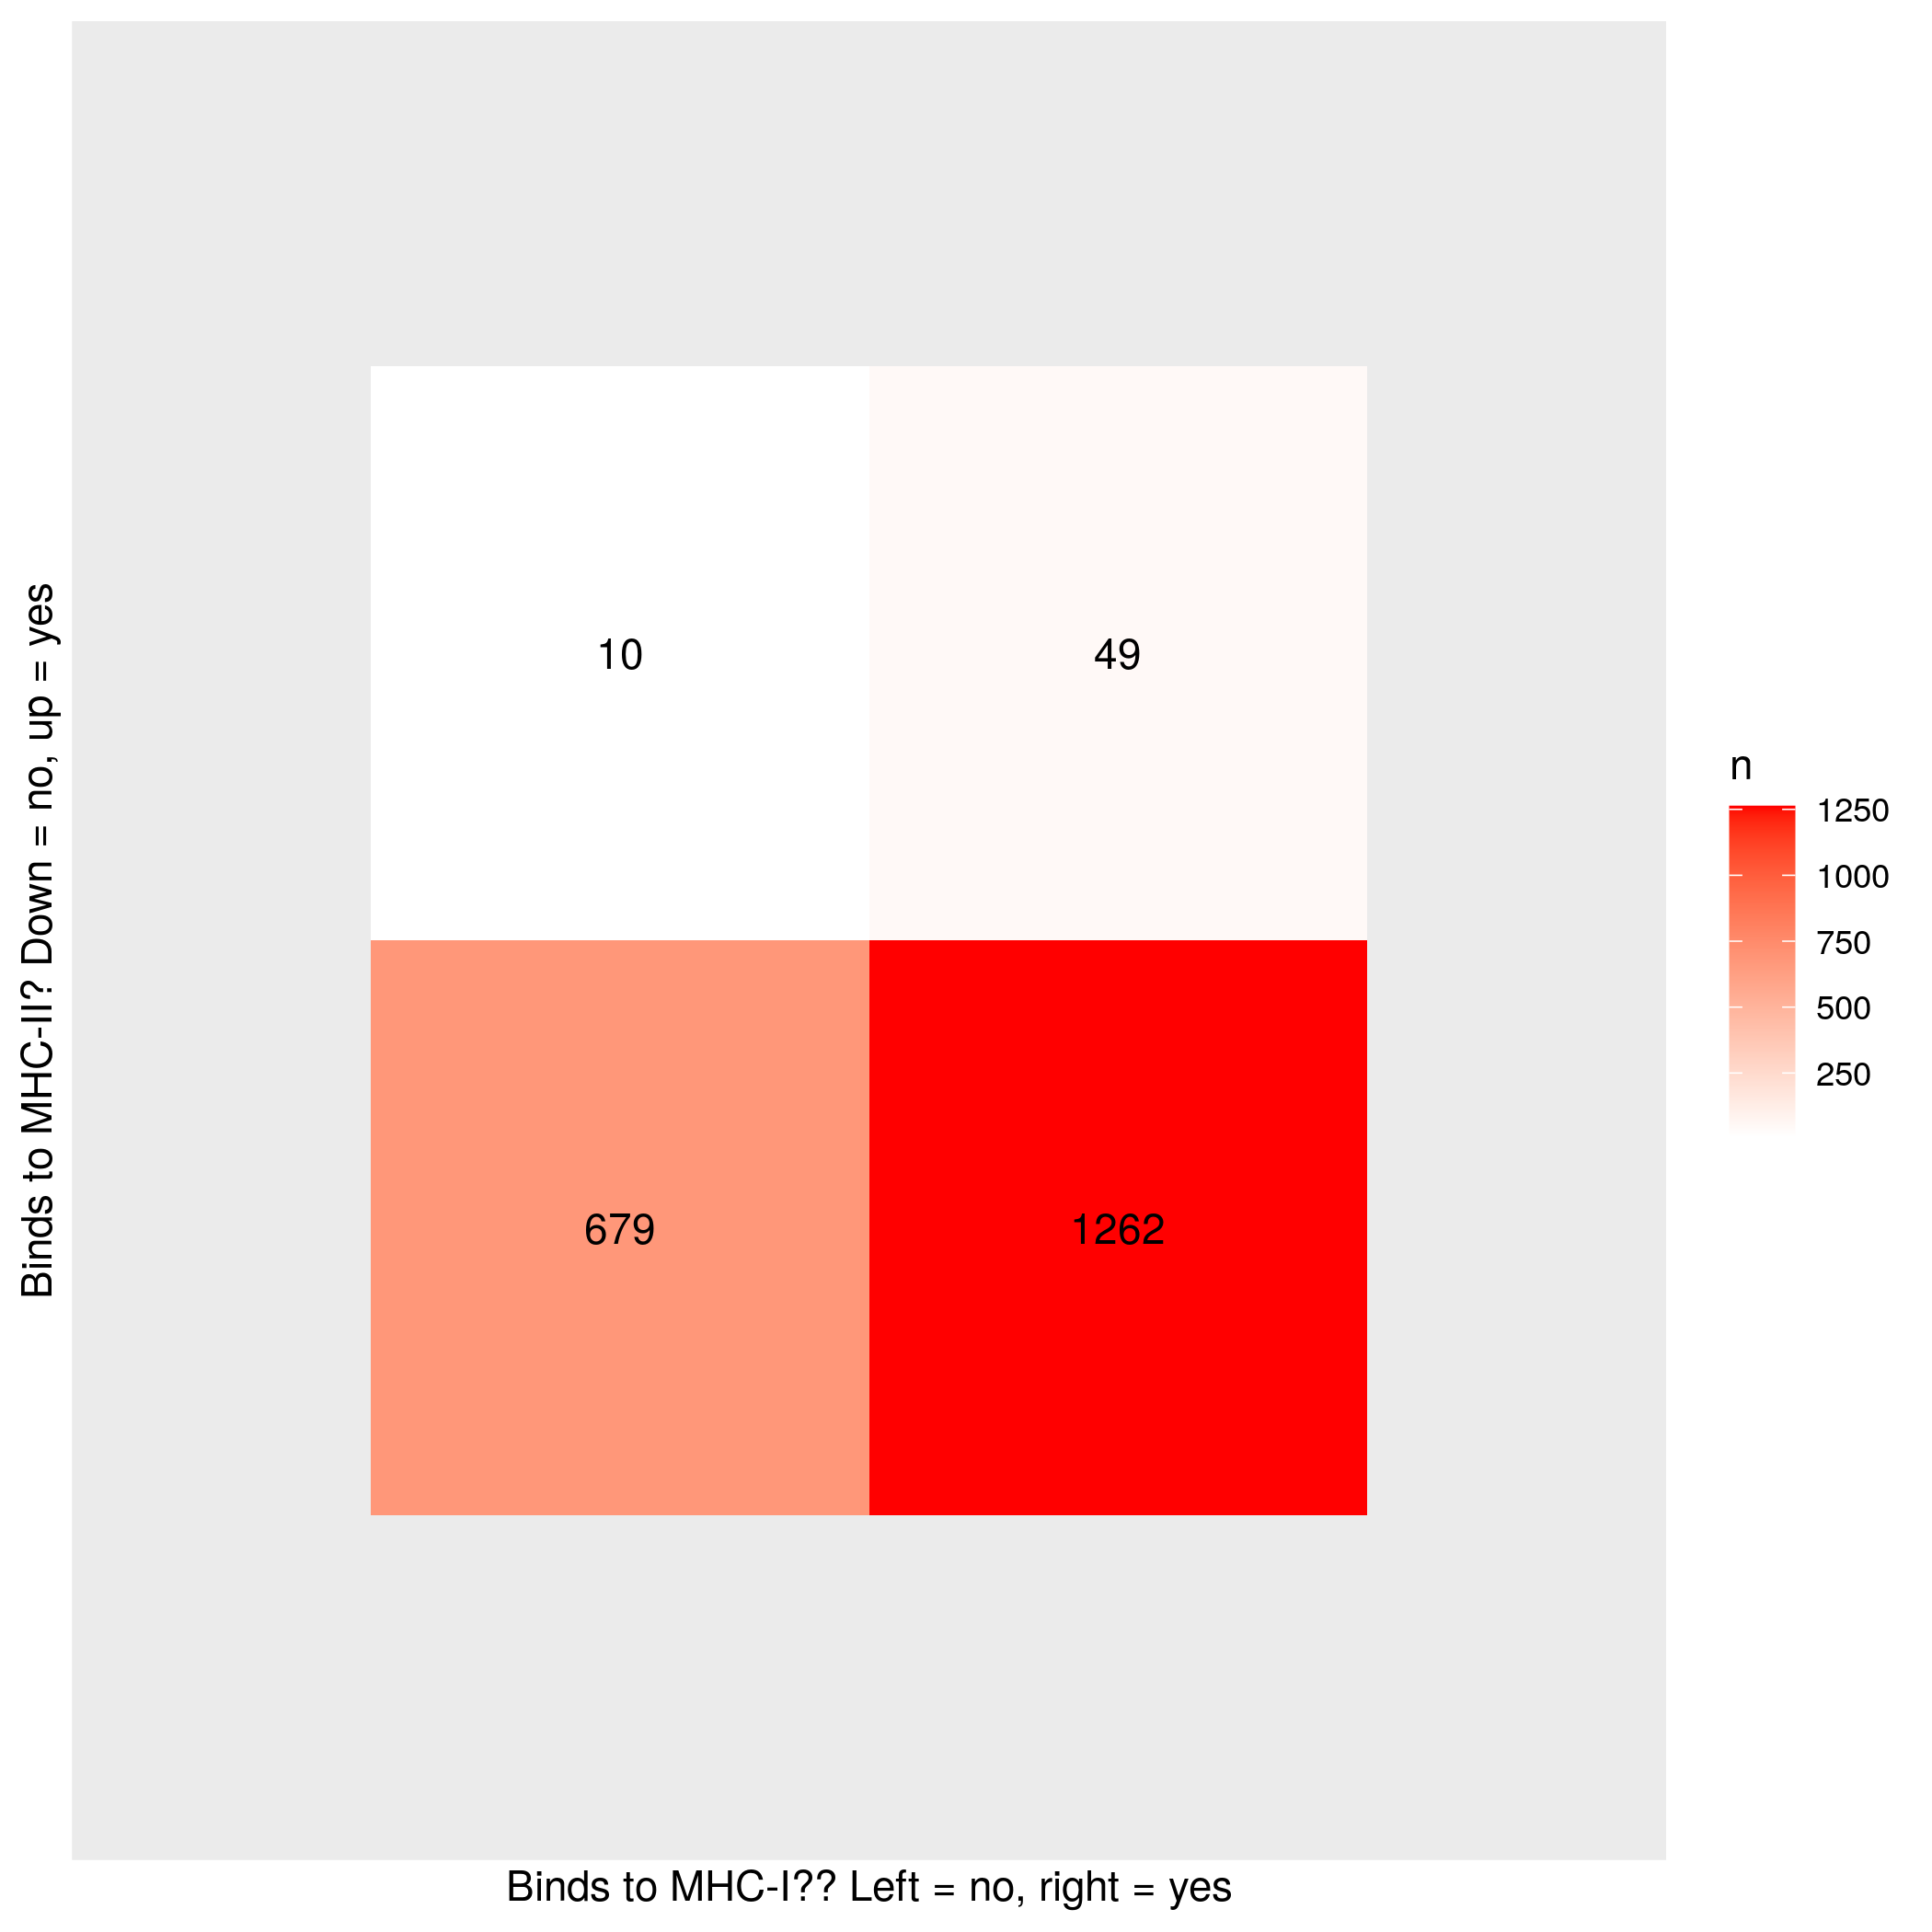
\includegraphics[width=0.9\textwidth]{p_bind_per_hydrophobicity/binds_mhc1_vs_binds_mhc2.png}
%  \caption{
%    \richel{Used randomly simulated peptides, results are real}
%  }
%  \label{fig:binds_mhc1_vs_binds_mhc2}
%\end{figure}

%\begin{figure}[!htbp]
%  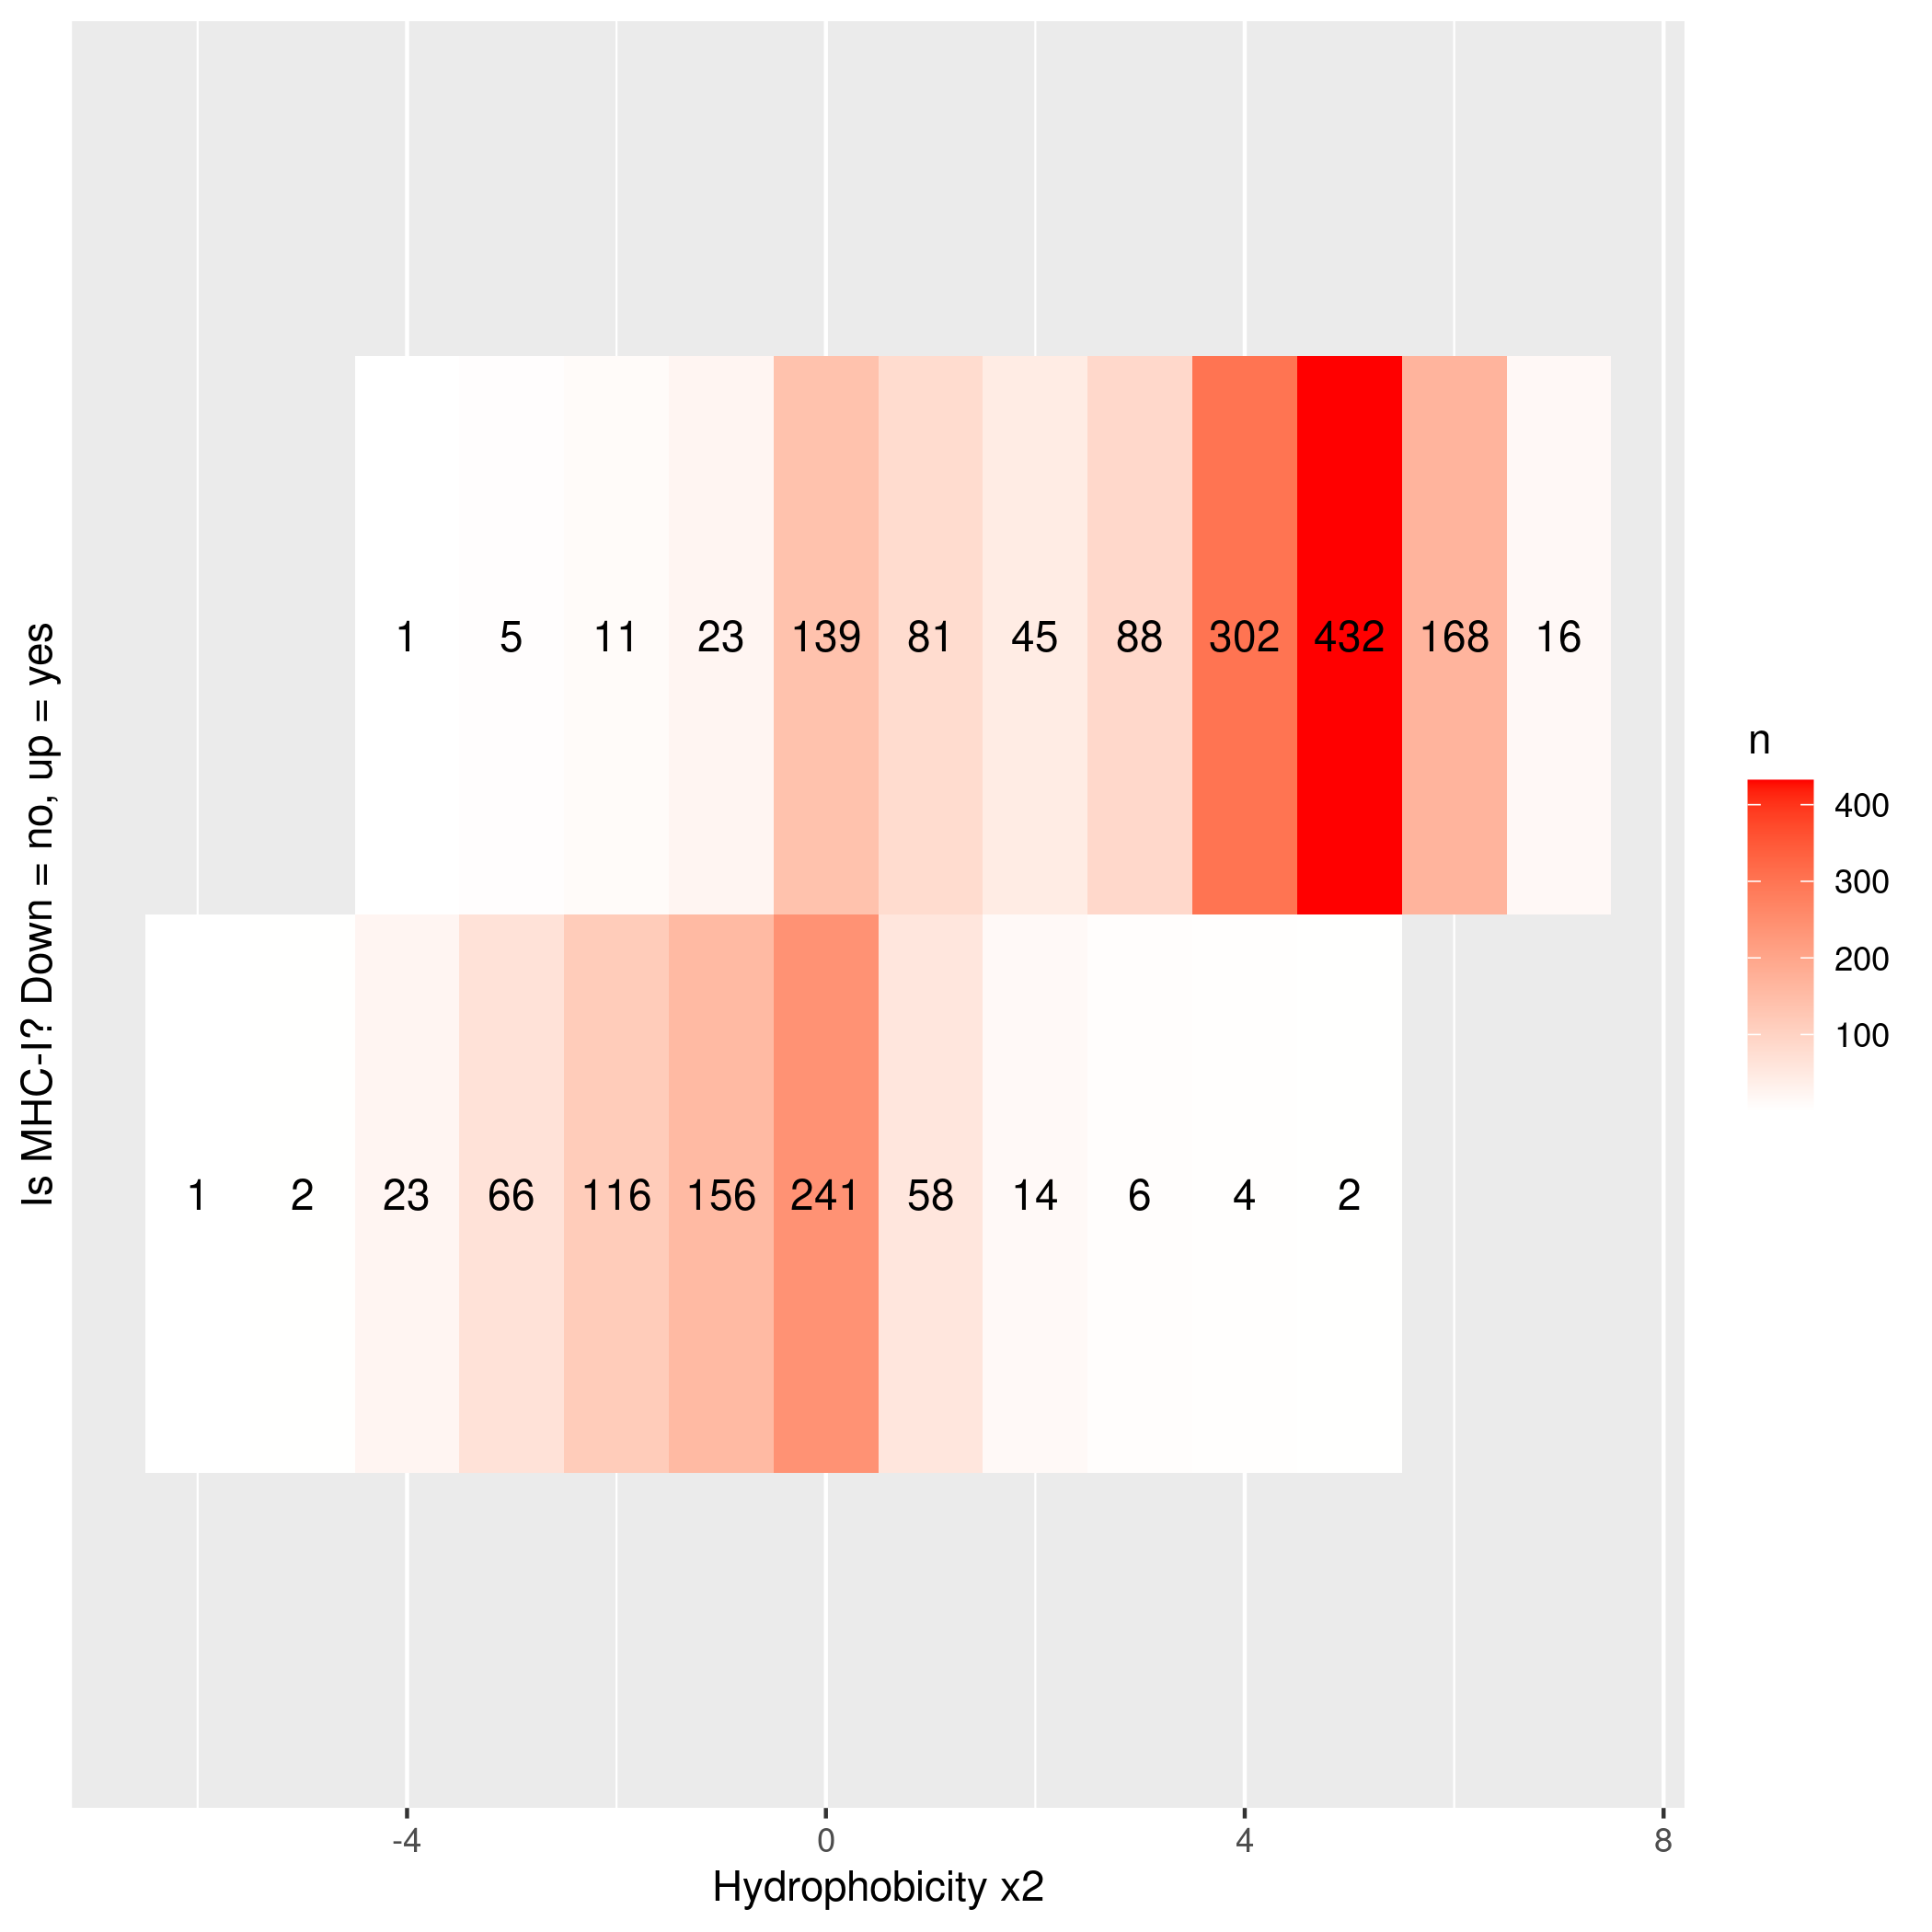
\includegraphics[width=0.9\textwidth]{p_bind_per_hydrophobicity/hydrophobicity_vs_binds_mhc1.png}
%  \caption{
%    \richel{Used randomly simulated peptides, results are real}
%  }
%  \label{fig:hydrophobicity_vs_binds_mhc1}
%\end{figure}

%\begin{figure}[!htbp]
%  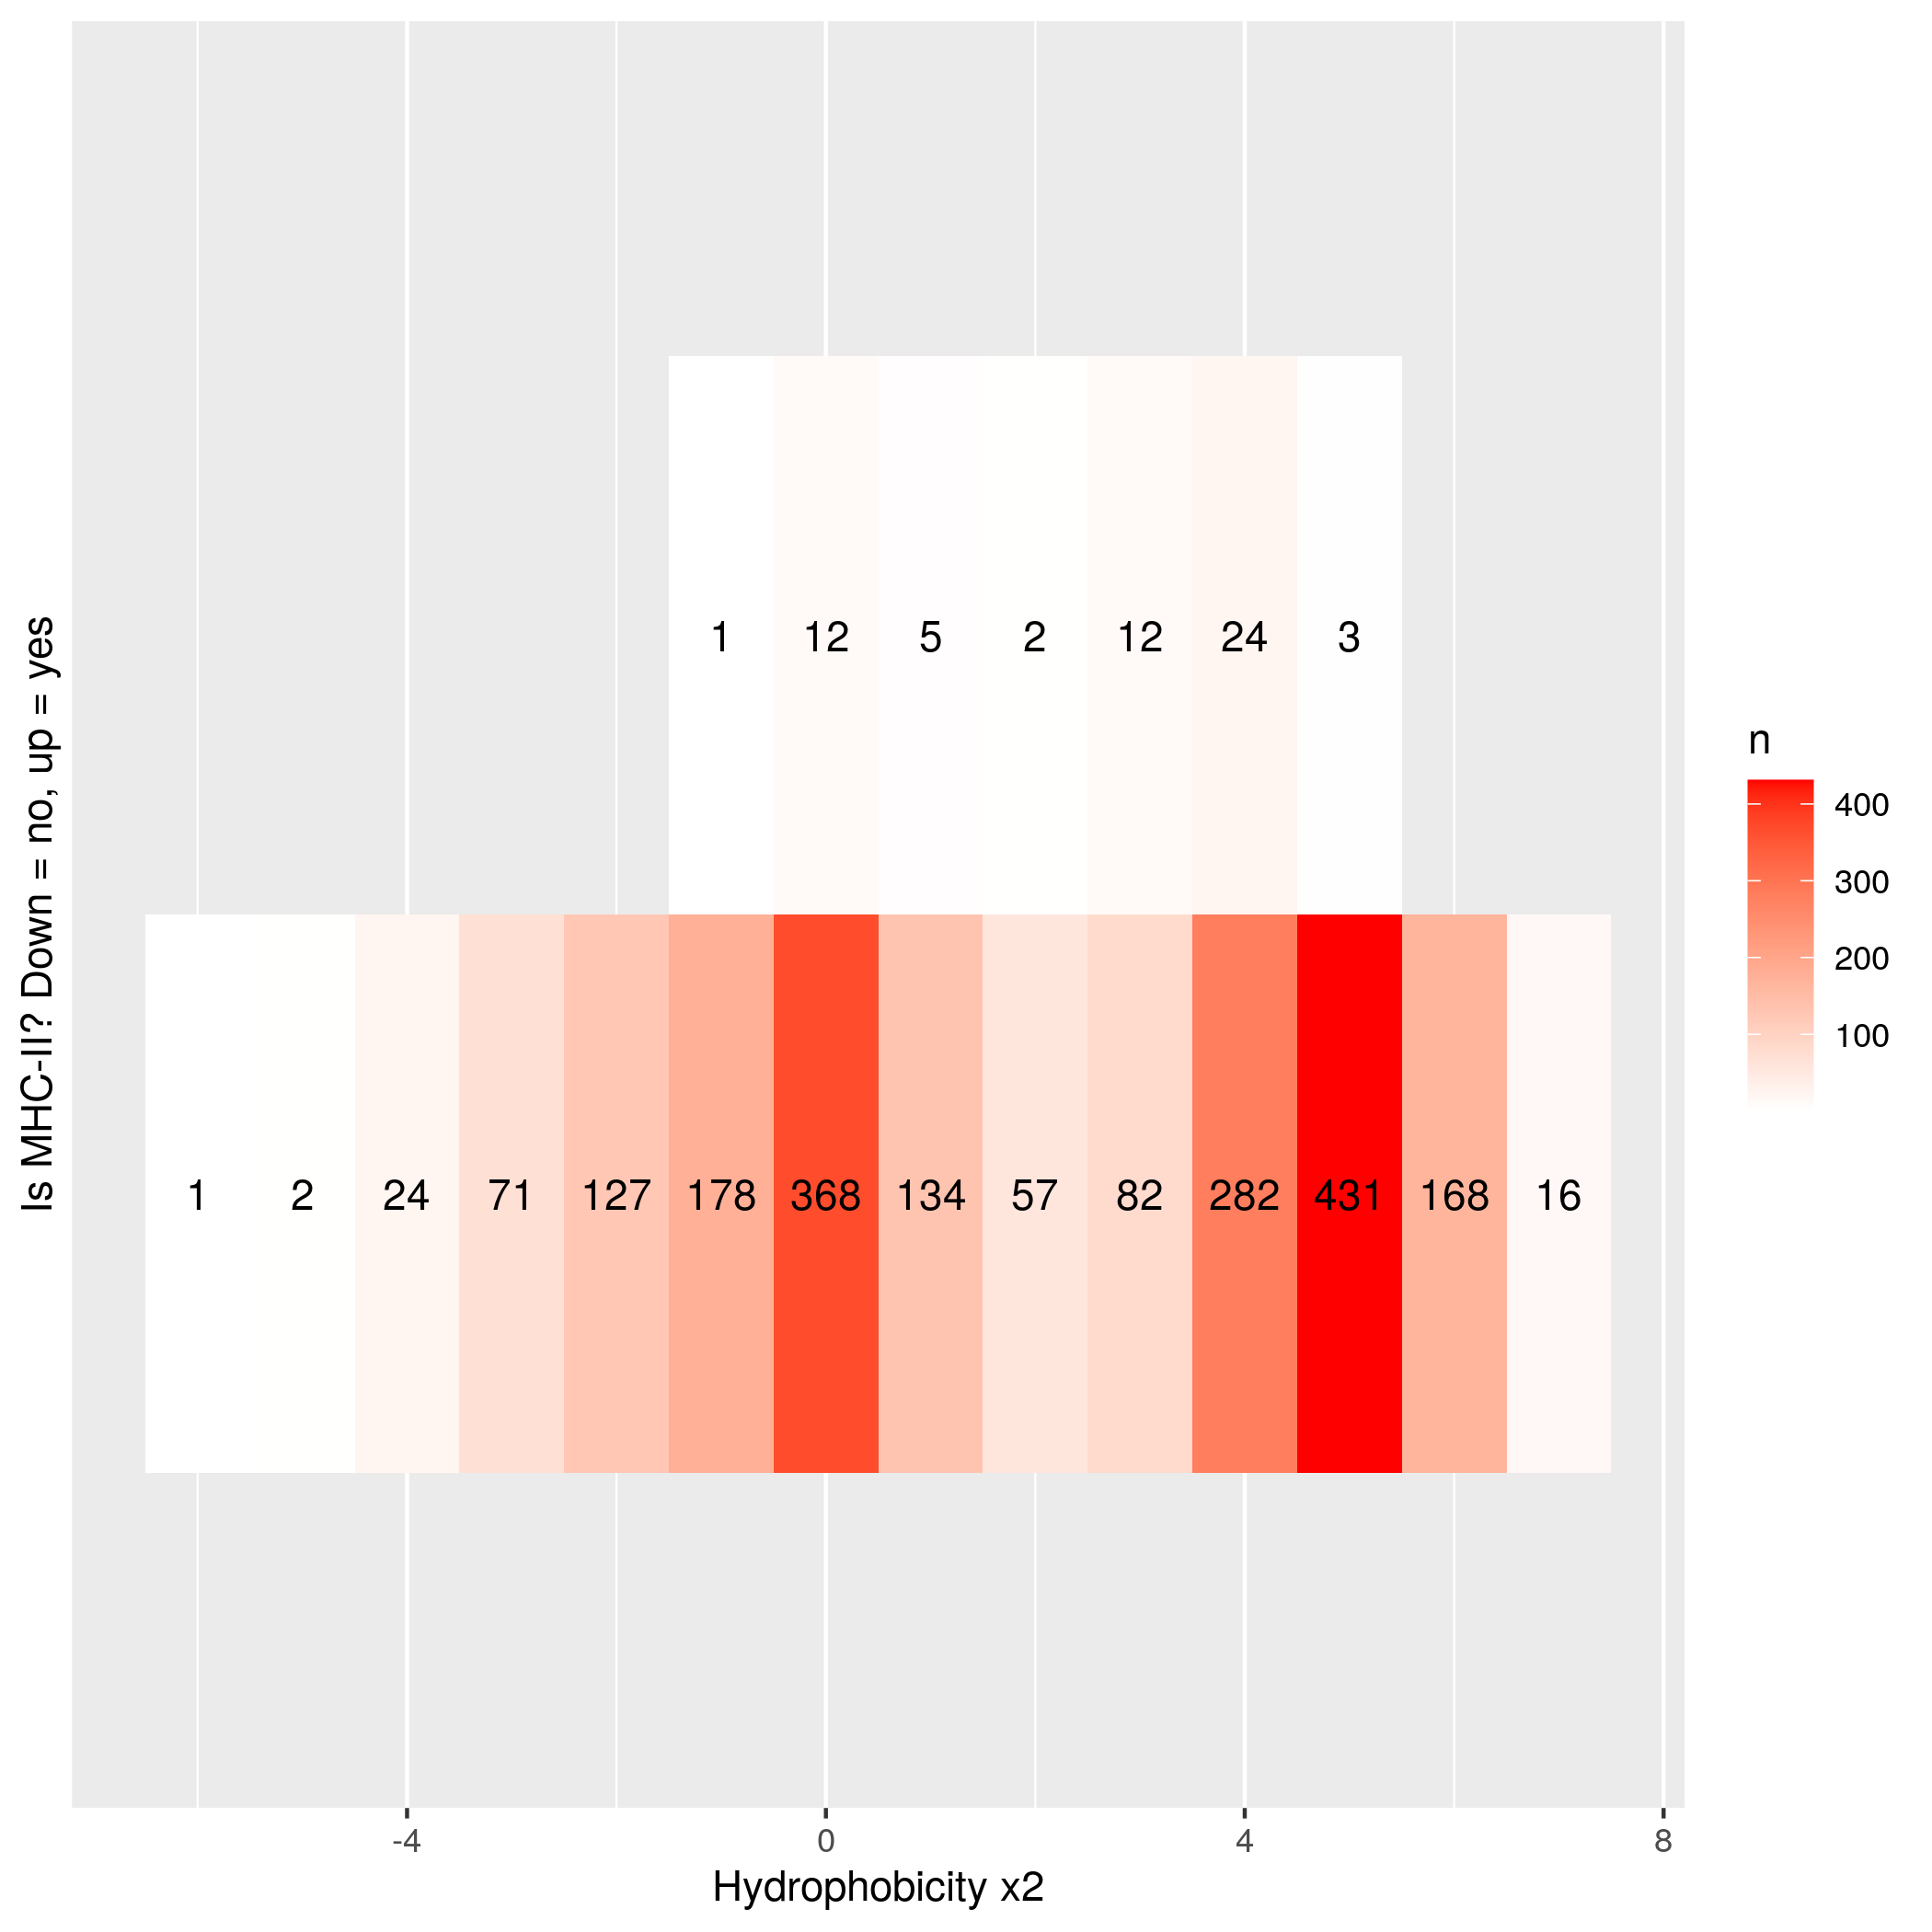
\includegraphics[width=0.9\textwidth]{p_bind_per_hydrophobicity/hydrophobicity_vs_binds_mhc2.png}
%  \caption{
%    \richel{Used randomly simulated peptides, results are real}
%  }
%  \label{fig:hydrophobicity_vs_binds_mhc2}
%\end{figure}

%\begin{figure}[!htbp]
%  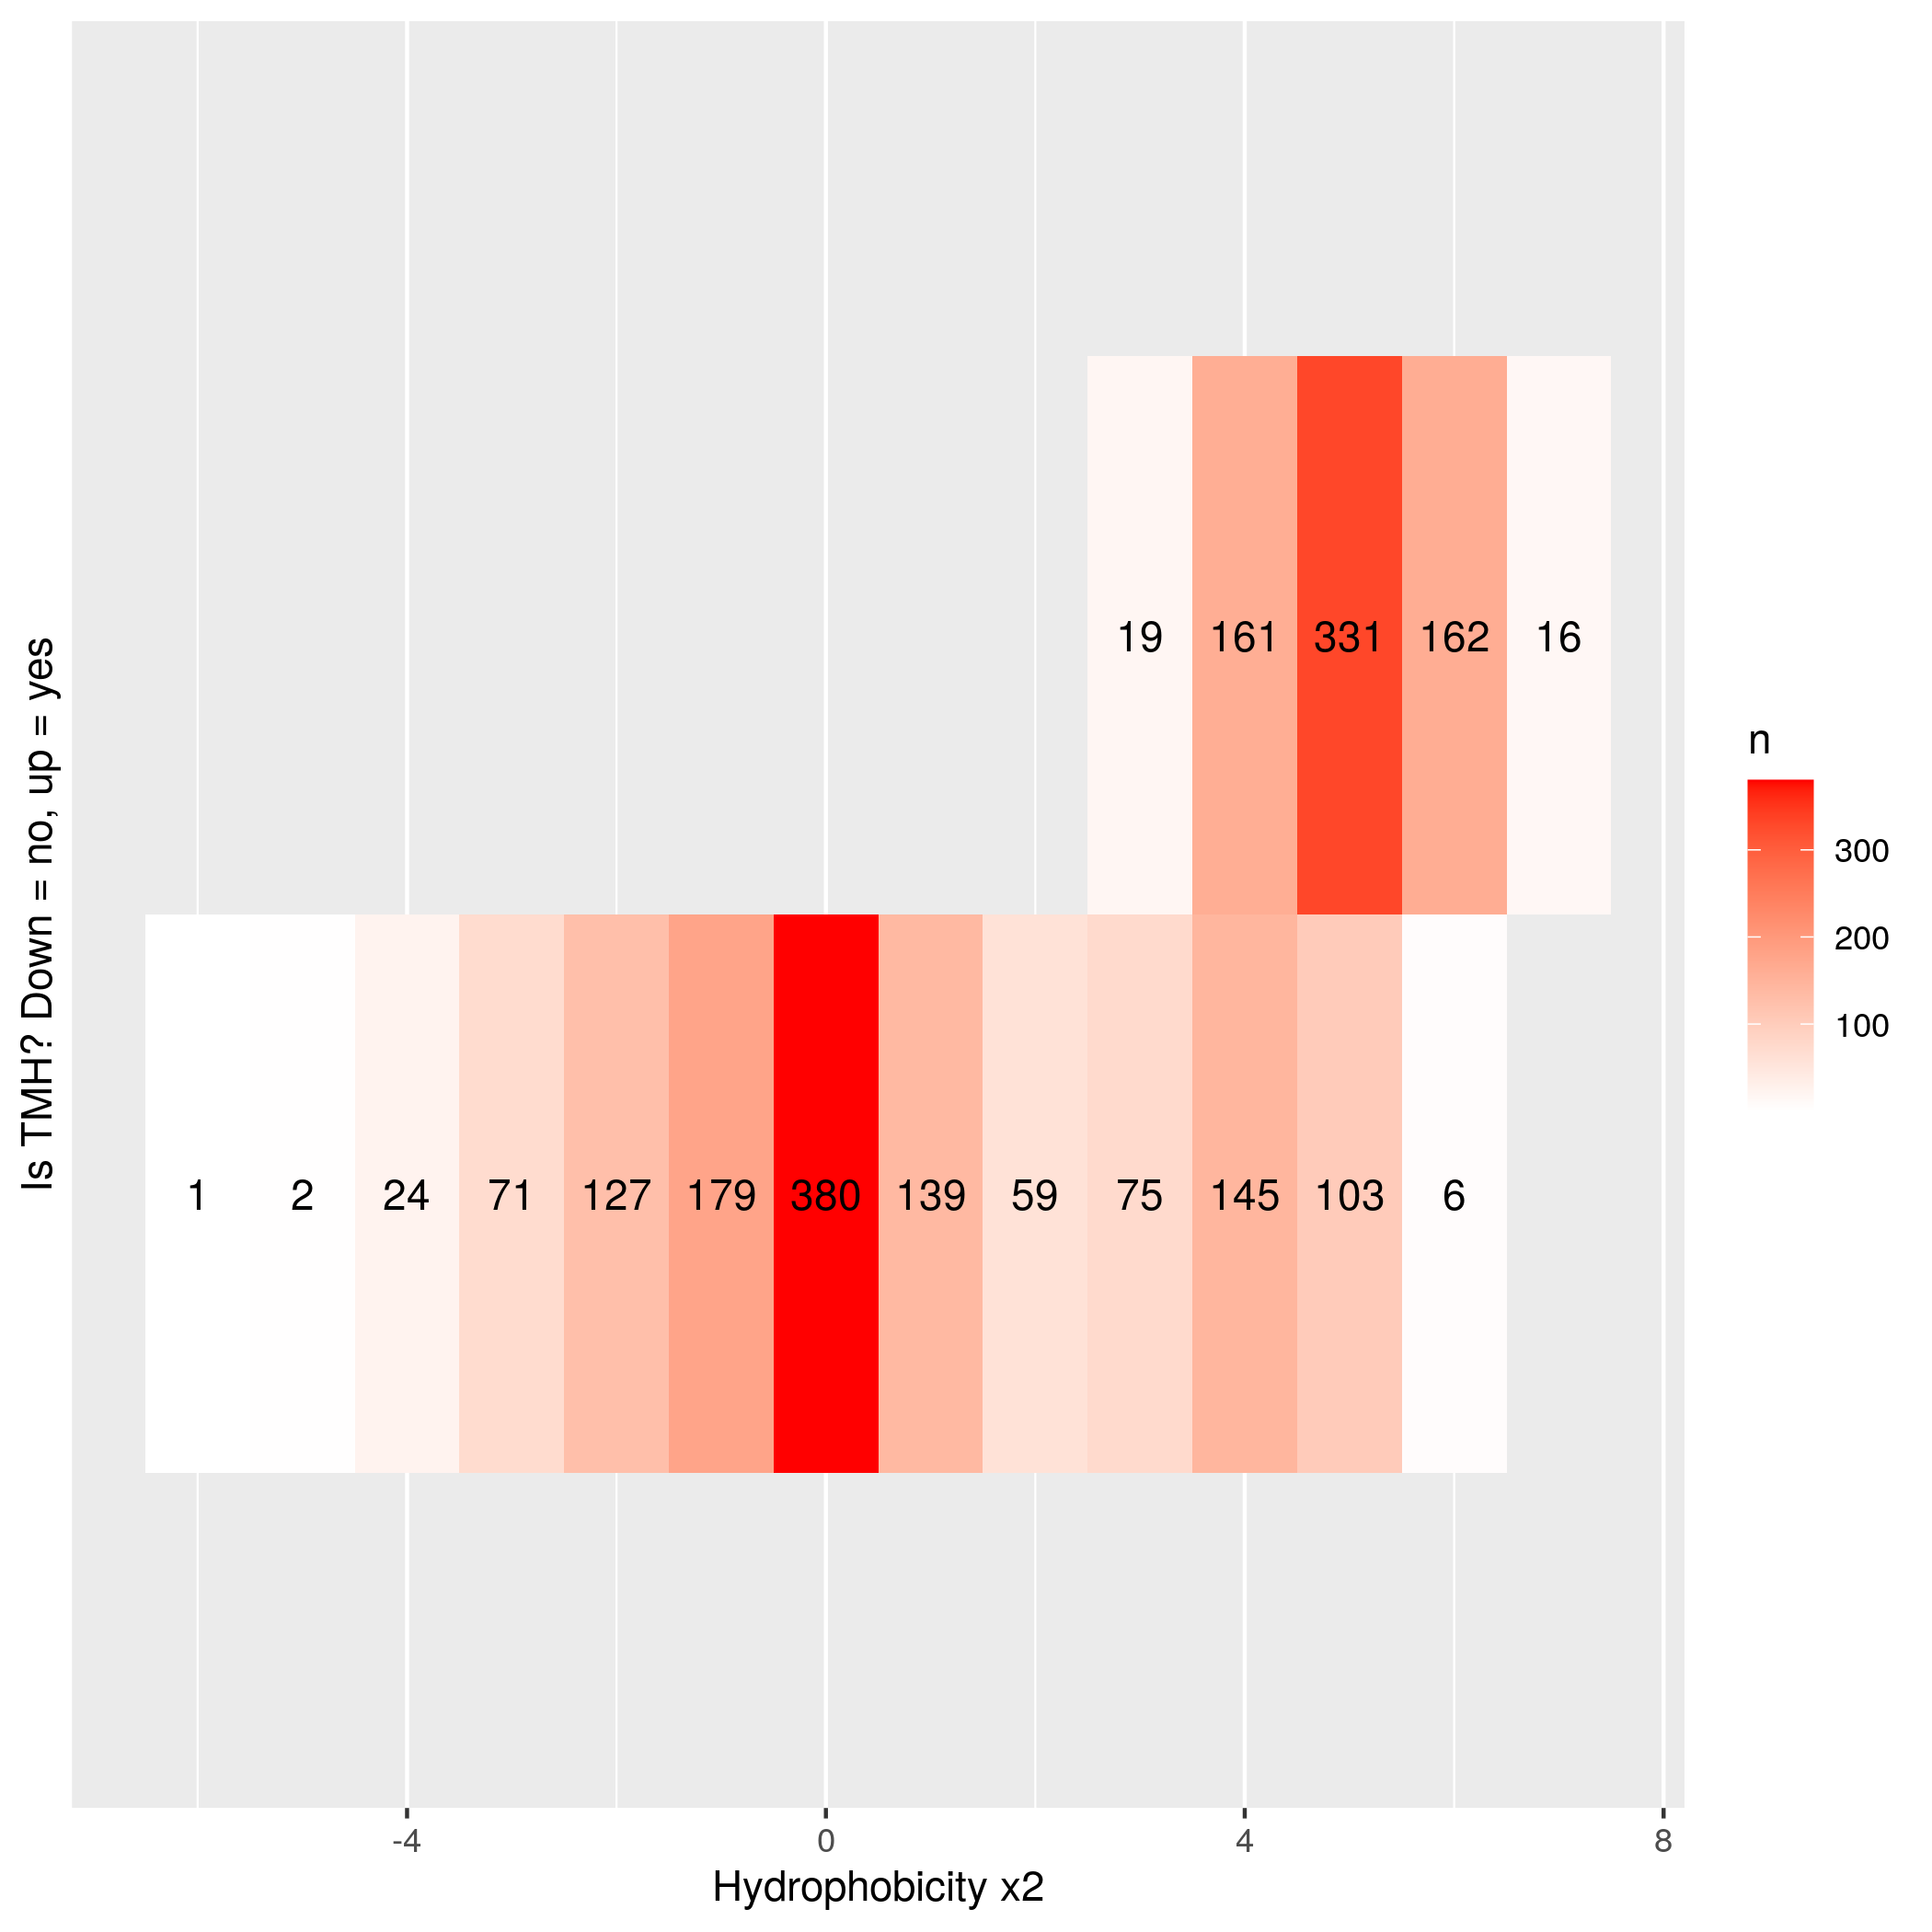
\includegraphics[width=0.9\textwidth]{p_bind_per_hydrophobicity/hydrophobicity_vs_is_tmh.png}
%  \caption{
%    \richel{Used randomly simulated peptides, results are real}
%  }
%  \label{fig:hydrophobicity_vs_is_tmh}
%\end{figure}

%\begin{figure}[!htbp]
%  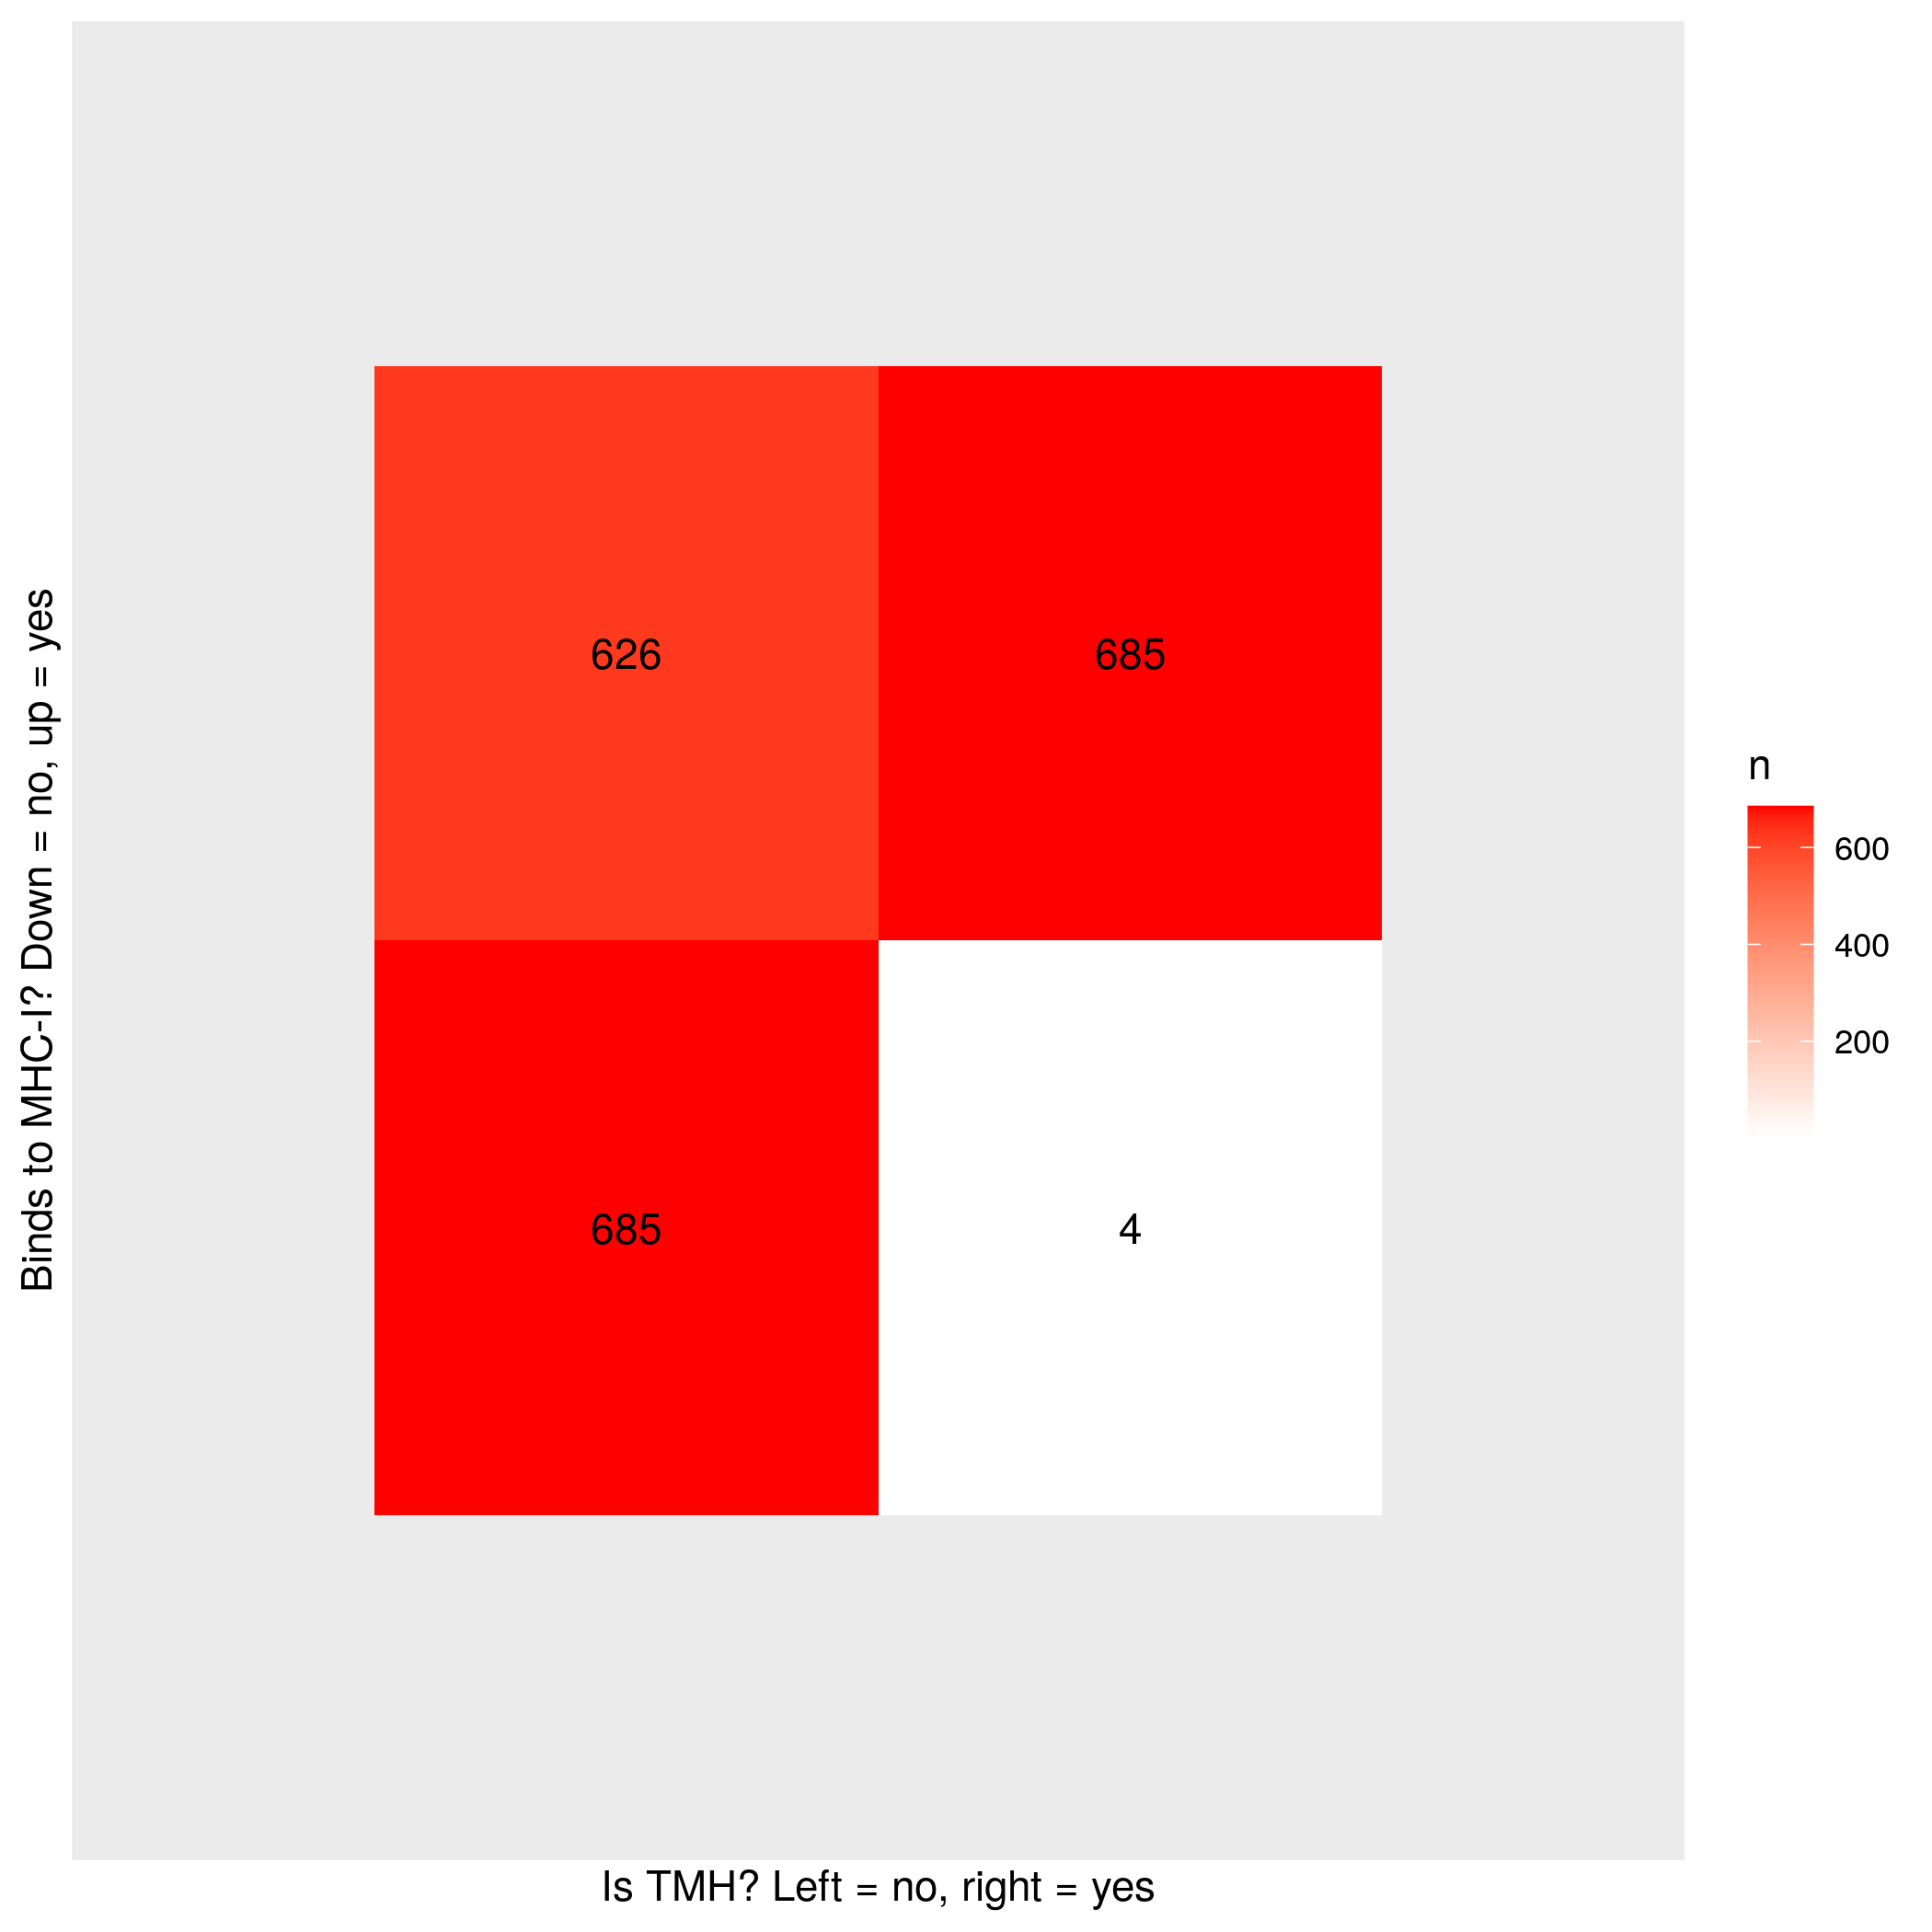
\includegraphics[width=0.9\textwidth]{p_bind_per_hydrophobicity/is_tmh_vs_binds_mhc1.png}
%  \caption{
%    \richel{Used randomly simulated peptides, results are real}
%  }
%  \label{fig:is_tmh_vs_binds_mhc1}
%\end{figure}

%\begin{figure}[!htbp]
%  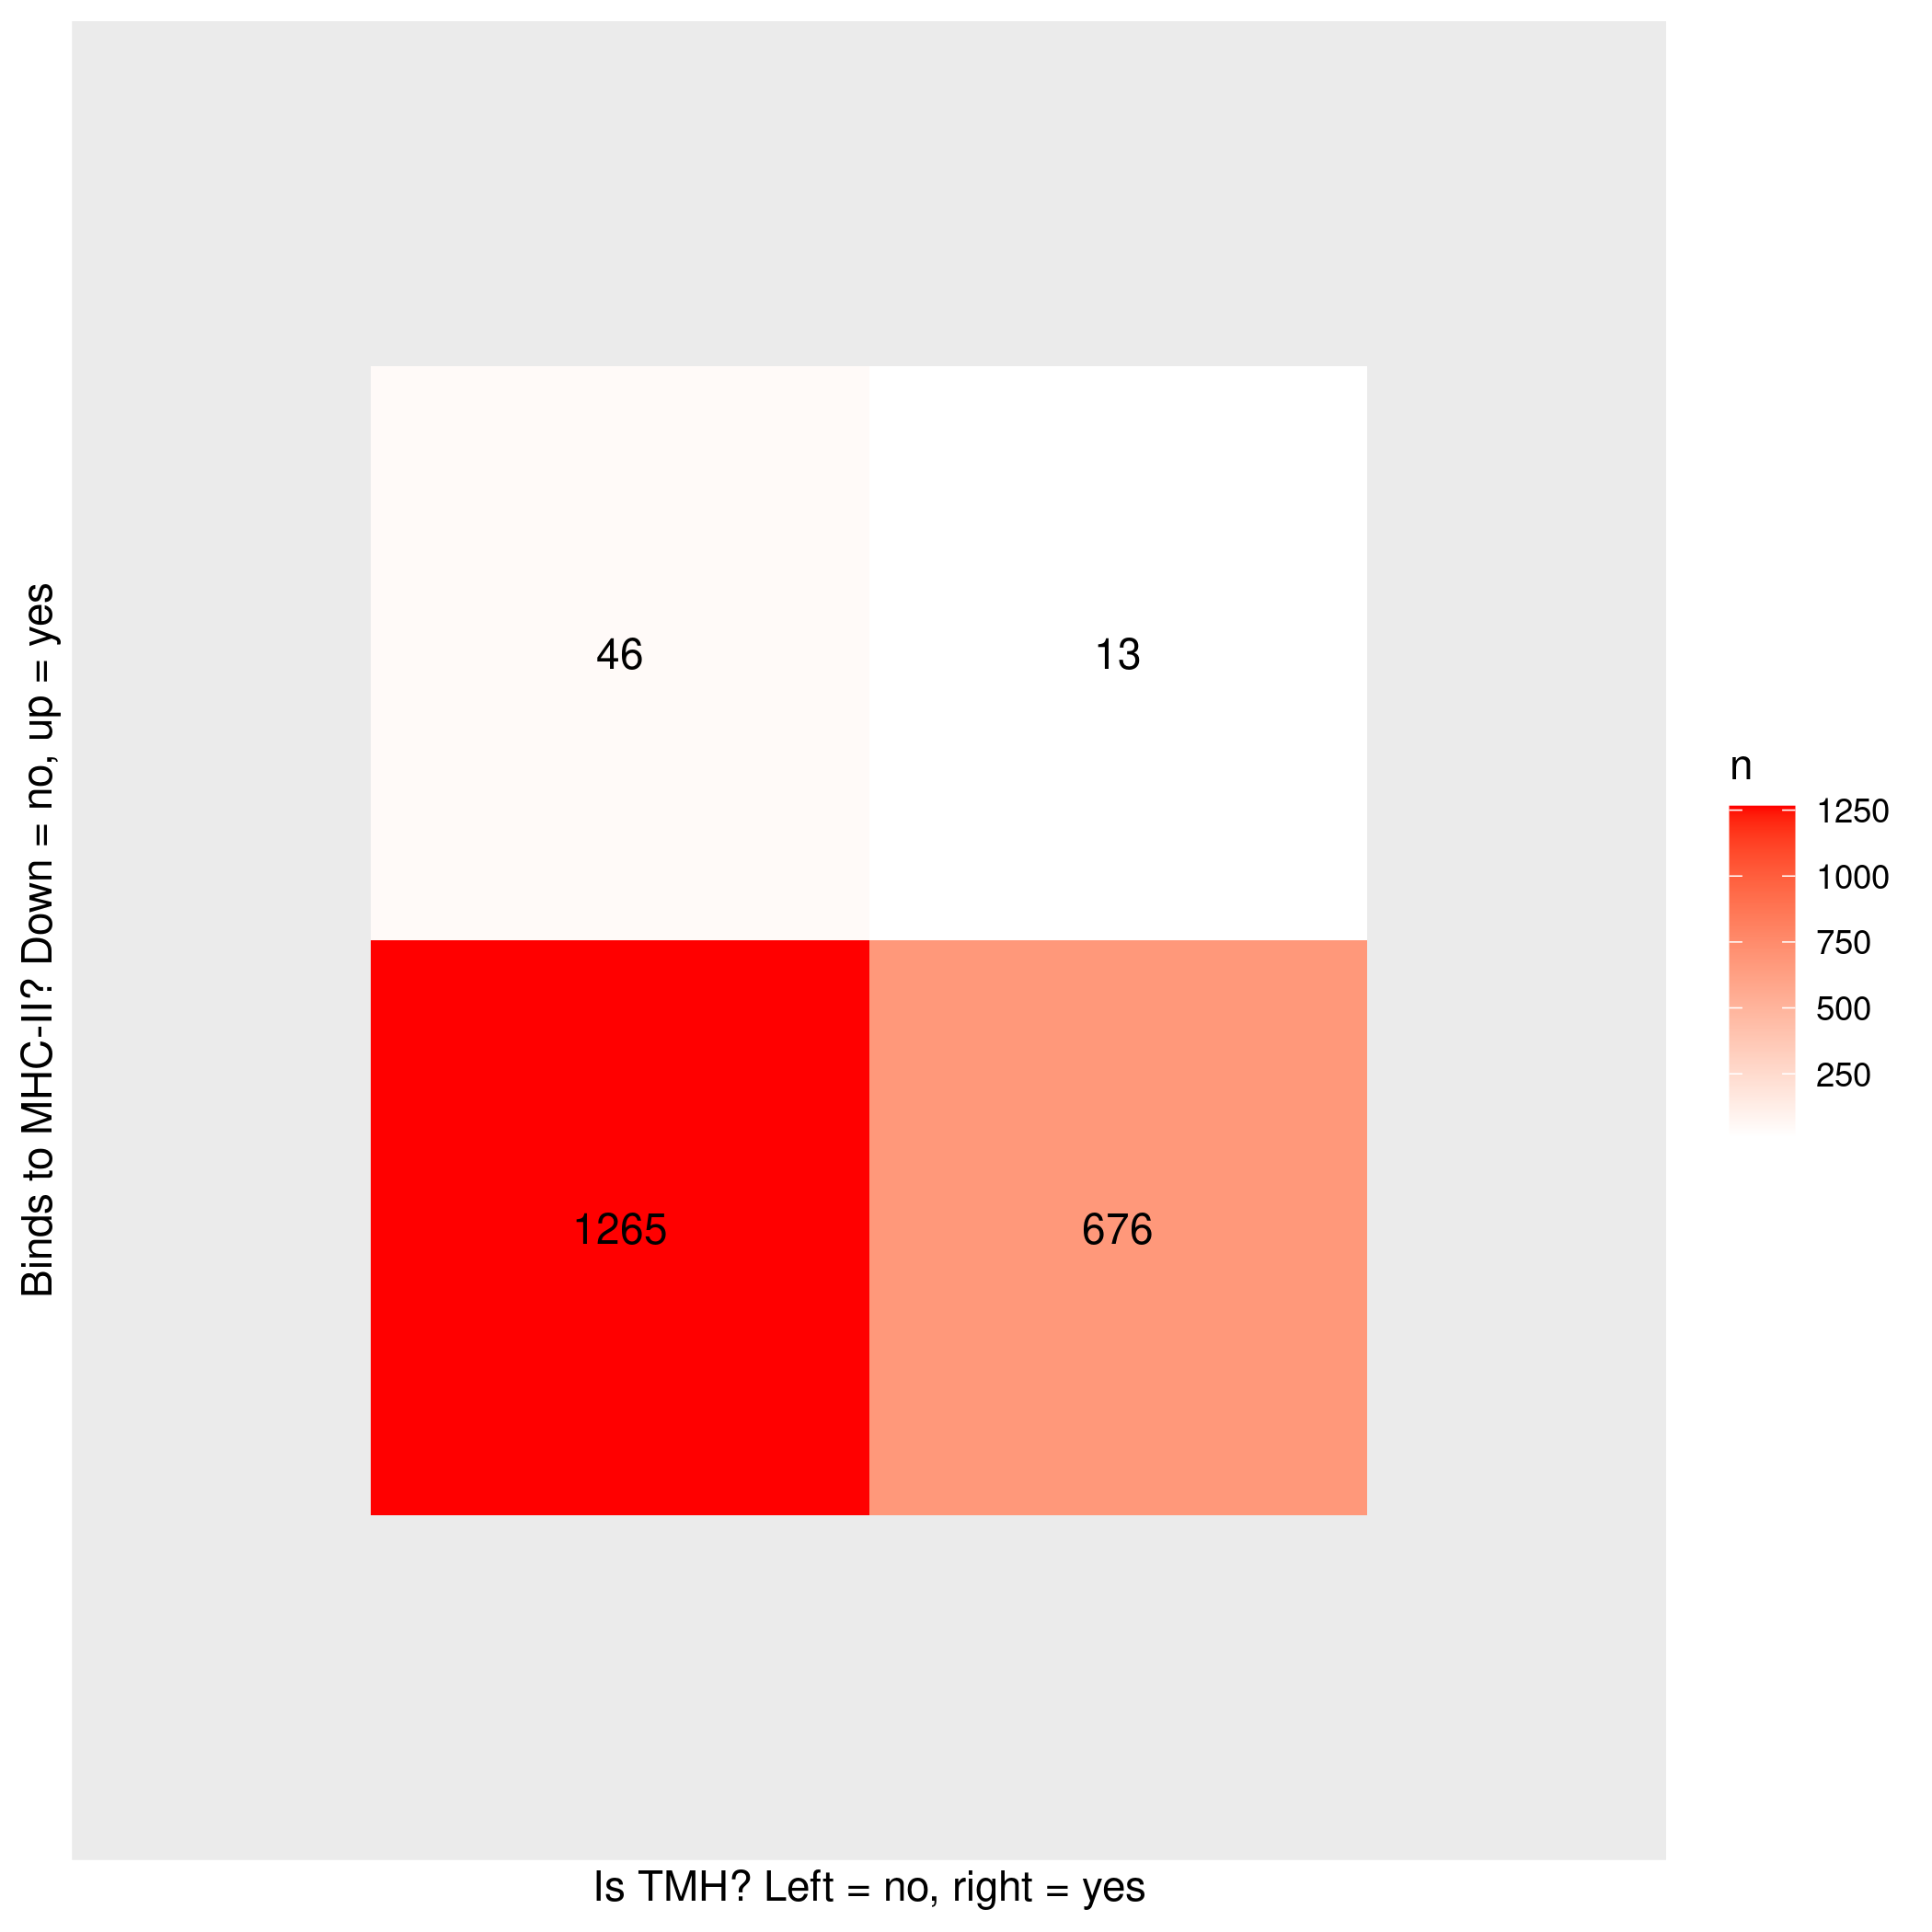
\includegraphics[width=0.9\textwidth]{p_bind_per_hydrophobicity/is_tmh_vs_binds_mhc2.png}
%  \caption{
%    \richel{Used randomly simulated peptides, results are real}
%  }
%  \label{fig:is_tmh_vs_binds_mhc2}
%\end{figure}

%%%%%%%%%%%%%%%%%%%%%%%%%%%%%%%%%%%%%%%%%%%%%%%%%%%%%%%%%%%%%%%%%%%%%%%%%%%%%%%%
\subsection{MHC-II haplotype occurrences}
%%%%%%%%%%%%%%%%%%%%%%%%%%%%%%%%%%%%%%%%%%%%%%%%%%%%%%%%%%%%%%%%%%%%%%%%%%%%%%%%

\begin{table}[!htbp]
  \input{mhc2_haplotypes.latex}
  \caption{
    Percentage of MHC-II haplotypes, from \cite{greenbaum2011functional}
  }
  \label{table:mhc2_haplotypes}
\end{table}

%%%%%%%%%%%%%%%%%%%%%%%%%%%%%%%%%%%%%%%%%%%%%%%%%%%%%%%%%%%%%%%%%%%%%%%%%%%%%%%%
\subsection{Relation between haplotype frequency and TMH over-representation}
%%%%%%%%%%%%%%%%%%%%%%%%%%%%%%%%%%%%%%%%%%%%%%%%%%%%%%%%%%%%%%%%%%%%%%%%%%%%%%%%

There is no relation between haplotype frequency and TMH over-representation.

\begin{figure}[!htbp]
  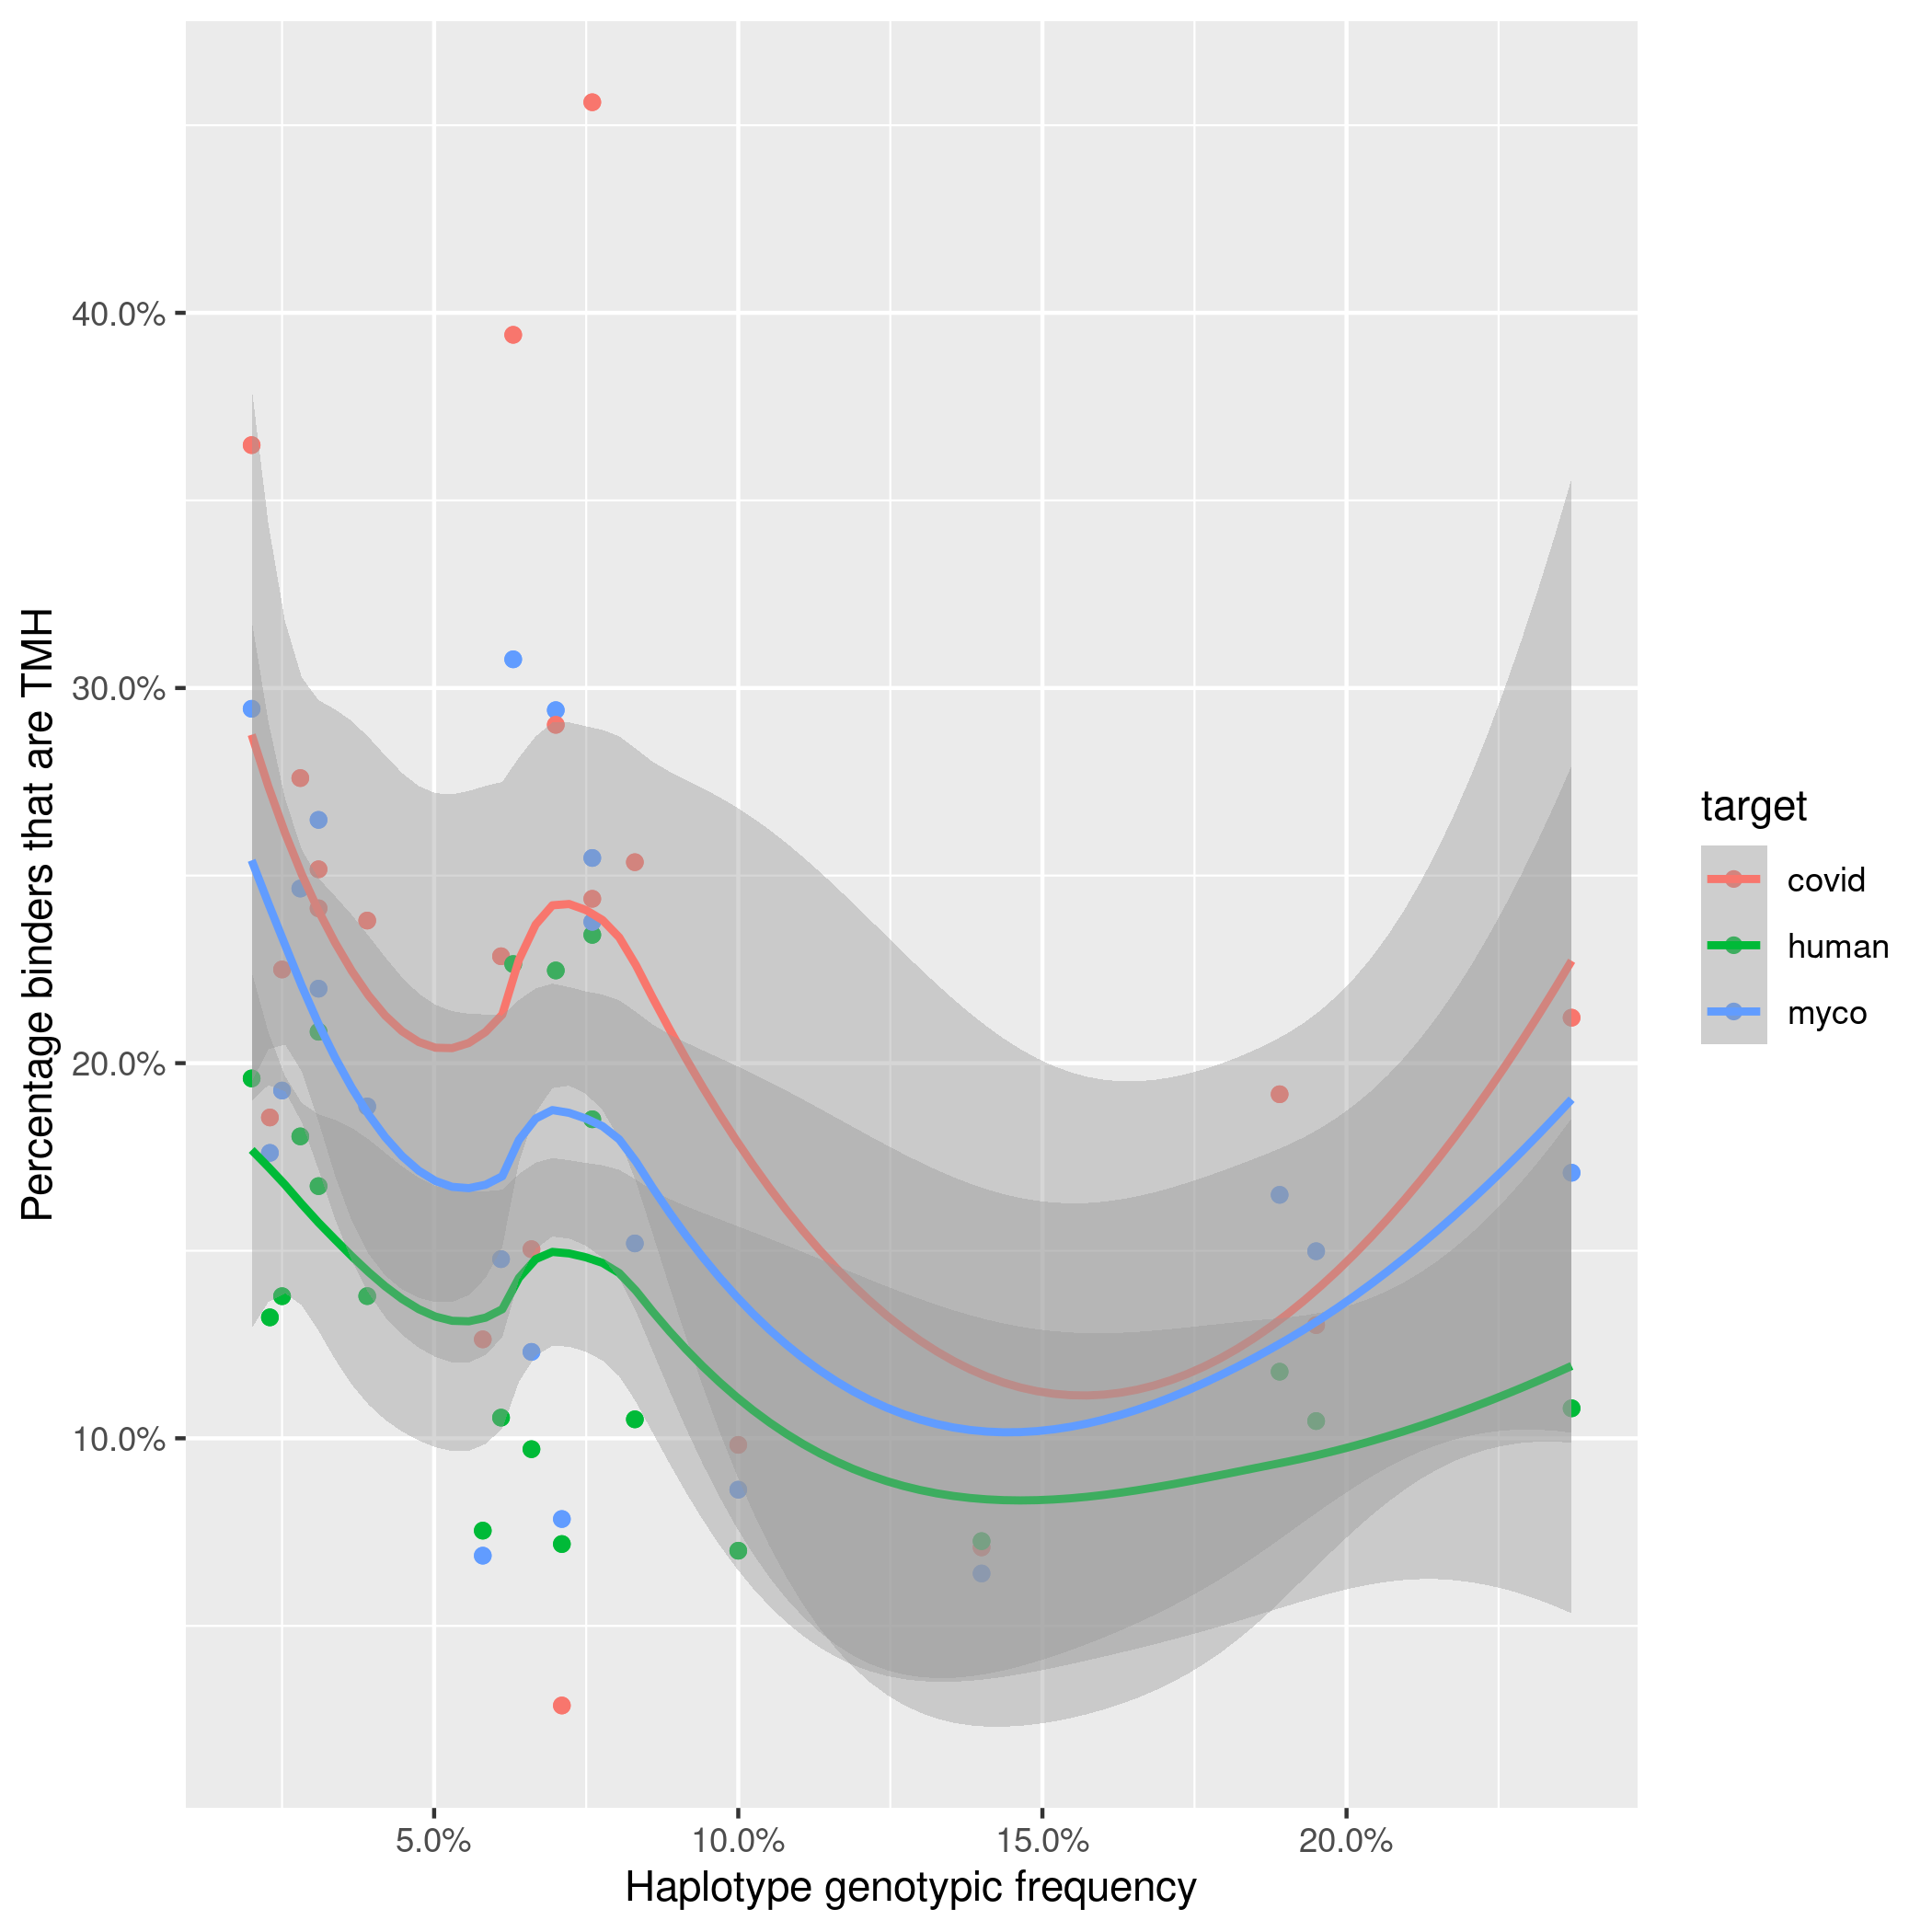
\includegraphics[width=\textwidth]{haplotype_freq_vs_f_tmh_epitopes/haplotype_perc_vs_f_tmh_binders.png}
  \caption{
    Relation between genotype frequency and the percentage
    of binders that are TMH for the 21 MHC-II haplotypes
  }
  \label{fig:haplotype_perc_vs_f_tmh_binders}
\end{figure}

\begin{figure}[!htbp]
  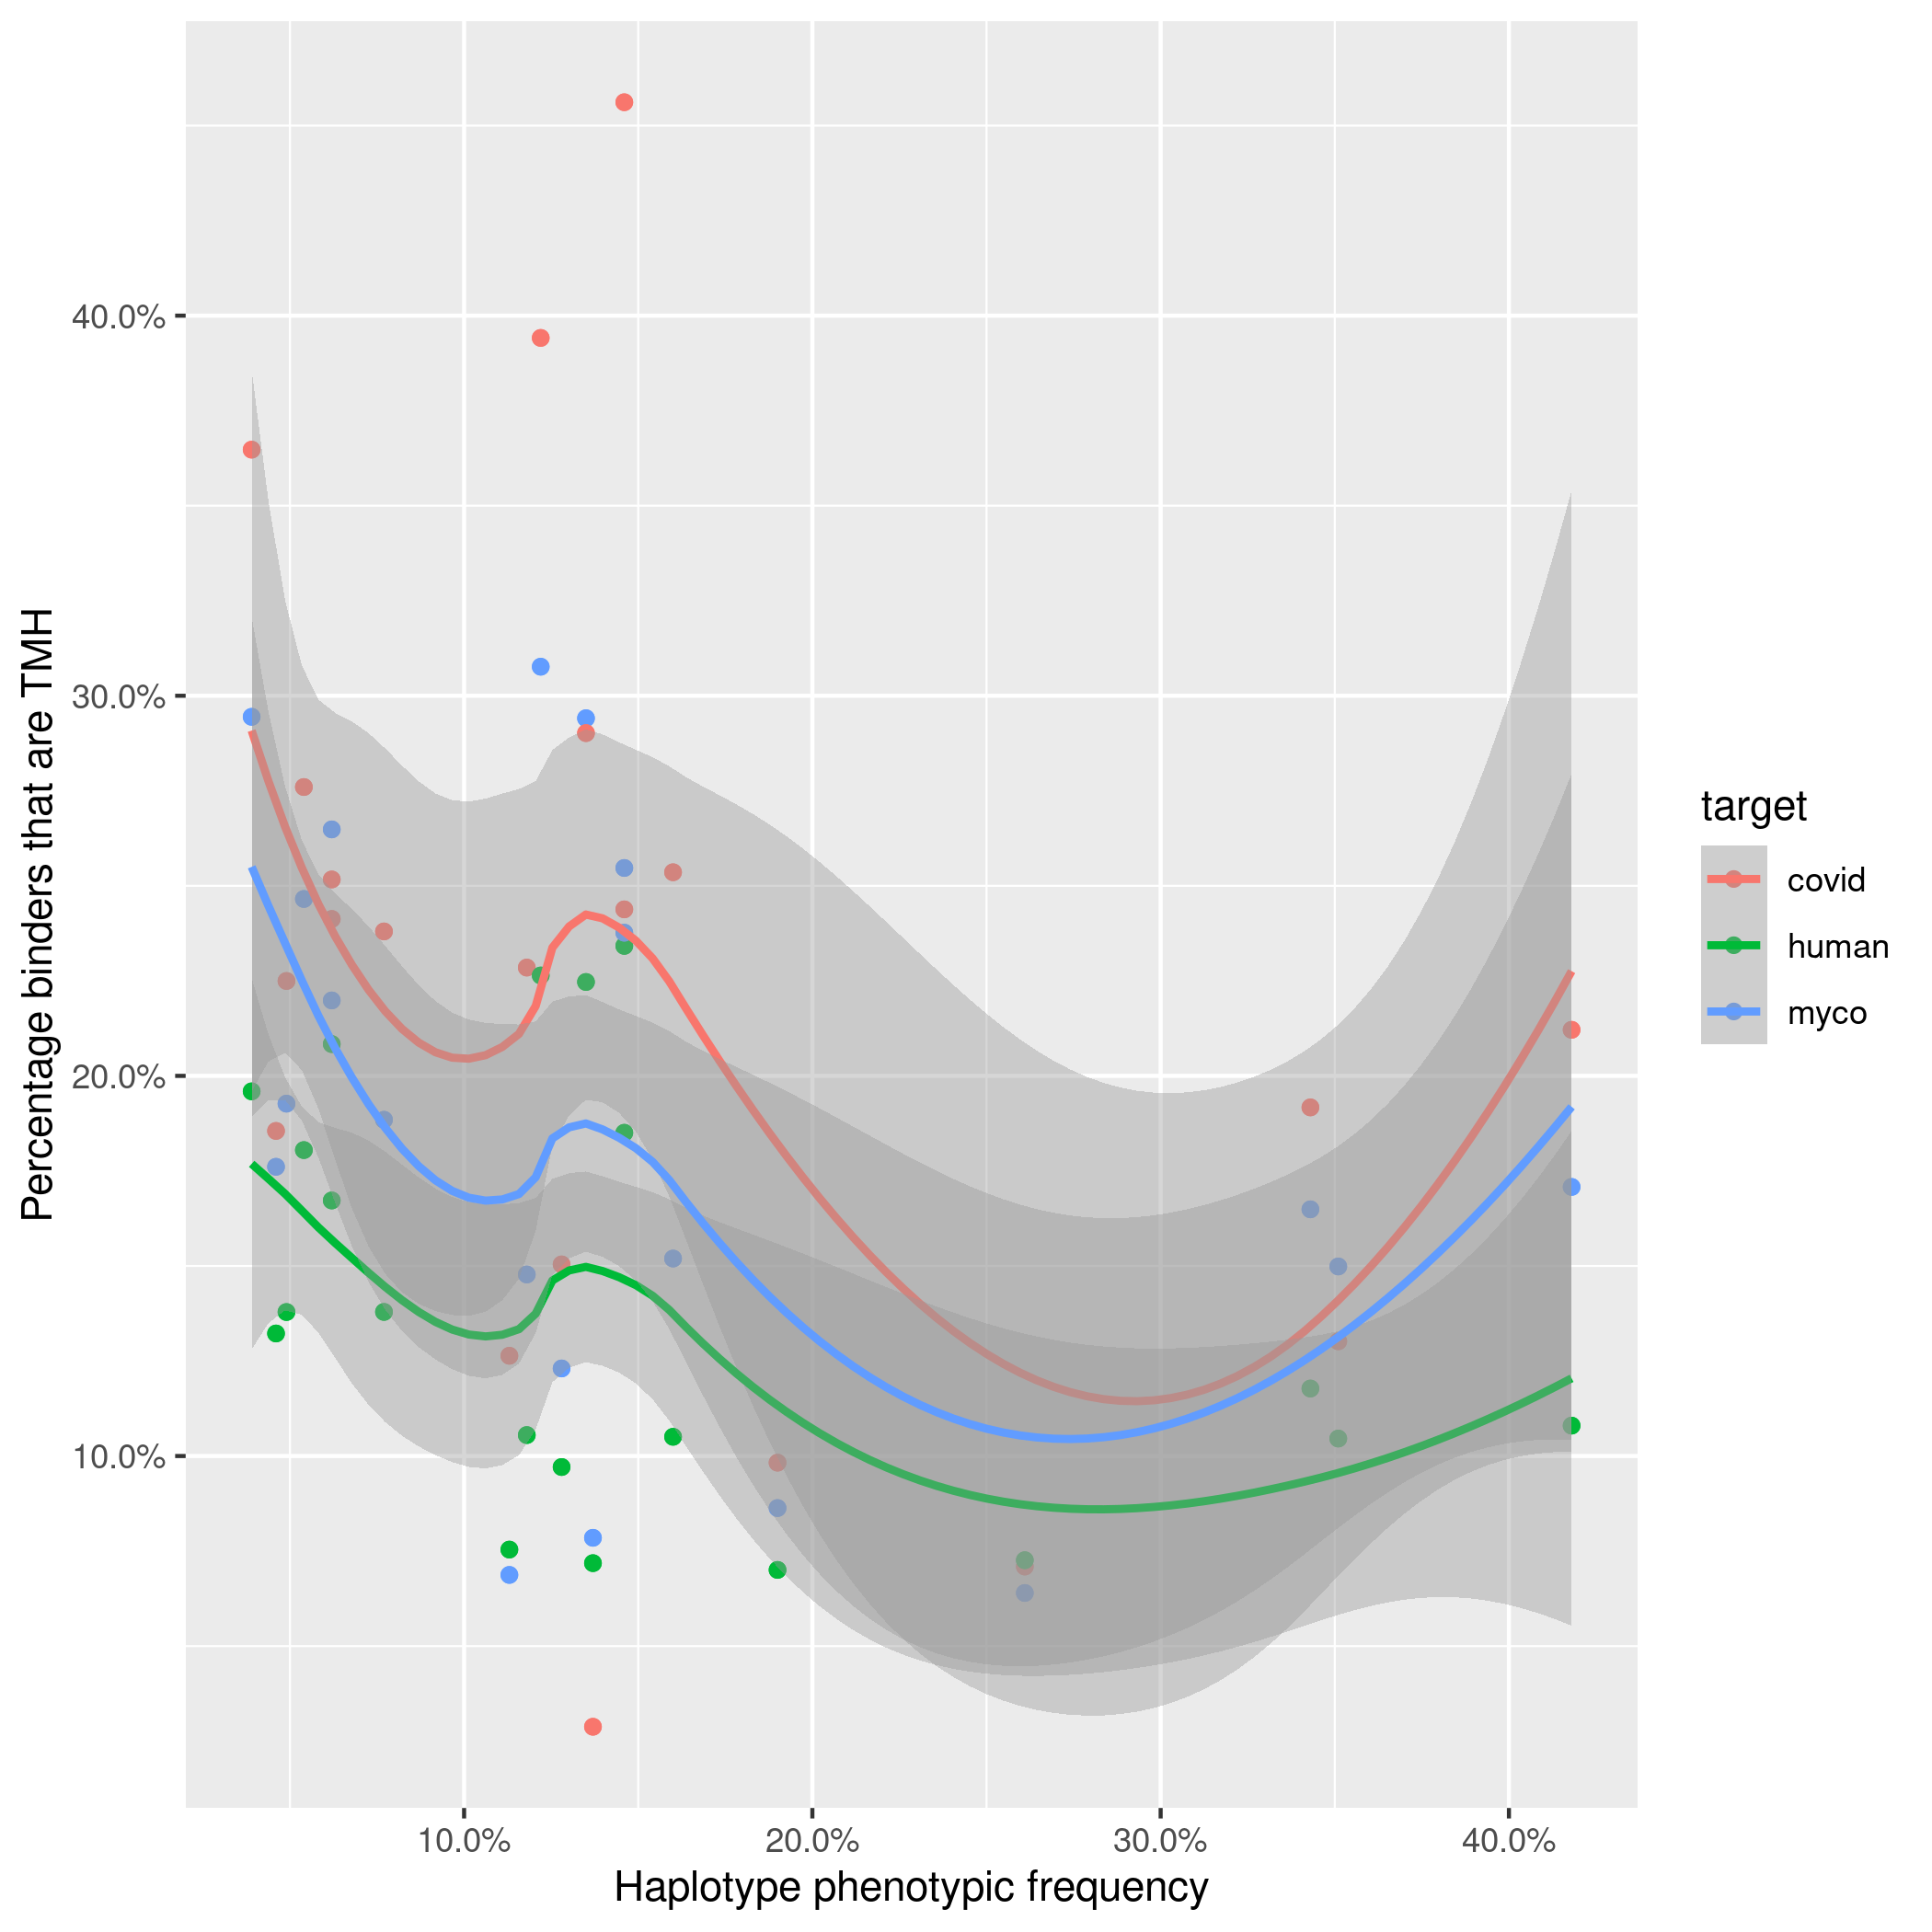
\includegraphics[width=\textwidth]{haplotype_freq_vs_f_tmh_epitopes/phenotype_freq_vs_f_tmh_binders.png}
  \caption{
    Relation between phenotype frequency and the percentage
    of binders that are TMH for the 21 MHC-II haplotypes
  }
  \label{fig:phenotype_freq_vs_f_tmh_binders}
\end{figure}

%%%%%%%%%%%%%%%%%%%%%%%%%%%%%%%%%%%%%%%%%%%%%%%%%%%%%%%%%%%%%%%%%%%%%%%%%%%%%%%%
\section{Hypotheses}
%%%%%%%%%%%%%%%%%%%%%%%%%%%%%%%%%%%%%%%%%%%%%%%%%%%%%%%%%%%%%%%%%%%%%%%%%%%%%%%%

\richel{As a reminder, to focus the research on}

\begin{itemize}
  \item $\mathcal{H}_{1,VB}$: MHC-I has the same percentage of epitopes overlapping
    with viral/bacterial TMHs as with human TMHs
  \item $\mathcal{H}_{2,HVB}$: MHC-II has the same percentage of epitopes overlapping
    with human/viral/bacterial TMHs as expected by chance
  \item $\mathcal{H}_{3}$: TMH and non-TMH regions are equally conserved
    in a proteome
\end{itemize}

